\documentclass[aspectratio=169]{beamer}
\usepackage[utf8]{inputenc}
\usepackage[T1]{fontenc}
\usepackage[brazil]{babel}
\usepackage{ragged2e}
\usepackage{booktabs}
\usepackage{verbatim}
\usetheme{AnnArbor}
\usecolortheme{orchid}
\usefonttheme[onlymath]{serif}
\usepackage{listings}
\usepackage{colortbl}
\usepackage{array}
\usepackage{xcolor}

\newcolumntype{C}[0]{>{\centering\arraybackslash}p{0.4cm}}

\lstset{language=C++,
	backgroundcolor=\color{green!10},
	basicstyle=\ttfamily,
	keywordstyle=\color{blue}\ttfamily,
	stringstyle=\color{red}\ttfamily,
	commentstyle=\color{green}\ttfamily,
	morecomment=[l][\color{magenta}]{\#},
	literate=
	{á}{{\'a}}1
	{à}{{\`a}}1
	{ã}{{\~a}}1
	{â}{{\^a}}1
	{é}{{\'e}}1
	{ê}{{\^e}}1
	{í}{{\'i}}1
	{ó}{{\'o}}1
	{õ}{{\~o}}1
	{ú}{{\'u}}1
	{ü}{{\"u}}1
	{ç}{{\c{c}}}1
	{Á}{{\'A}}1
	{À}{{\`A}}1
	{Ã}{{\~A}}1
	{Â}{{\^A}}1
	{É}{{\'E}}1
	{Ê}{{\^E}}1
	{Í}{{\'I}}1
	{Ó}{{\'O}}1
	{Õ}{{\~O}}1
	{Ú}{{\'U}}1
	{Ü}{{\"U}}1
	{Ç}{{\c{C}}}1
}

\lstdefinelanguage{XML}{
  showstringspaces=false,
  morestring=[b]",
  morestring=[s]{>}{<},
  morecomment=[s]{<?}{?>},
  stringstyle=\color{black},
  identifierstyle=\color{darkblue},
  keywordstyle=\color{cyan},
  morekeywords={xmlns,version,type}% list your attributes here
}

\AtBeginSection[]{
  \begin{frame}
  \vfill
  \centering
  \begin{beamercolorbox}[sep=8pt,center,shadow=true,rounded=true]{title}
    \usebeamerfont{title}\insertsectionhead\par%
  \end{beamercolorbox}
  \vfill
  \end{frame}
}

\title[\sc{Árvores}]{Árvores}
\author[Roland Teodorowitsch]{Roland Teodorowitsch}
\institute[ALEST I - EP - PUCRS]{Algoritmos e Estruturas de Dados I - Escola Politécnica - PUCRS}
\date{24 de outubro de 2023}

\begin{document}

\justifying

%-------------------------------------------------------
\begin{frame}
	\titlepage
\end{frame}

%=======================================================
\section{Introdução}

%-------------------------------------------------------
\begin{frame}\frametitle{Leitura(s) Recomendada(s)}

\begin{columns}[T]
\begin{column}{0.15\linewidth}
\vspace{-3mm}
\begin{figure}[h]
	\centering
	\includegraphics[height=0.3\paperheight]{imagens/livro_goodrich.jpg}
\end{figure}
\end{column}
%\vspace{3mm}
\begin{column}{0.85\linewidth}
\tiny{\textbf{Capítulo 7, Seções 7.1 e 7.2}\\
~}\\
\scriptsize{GOODRICH, Michael T.; TAMASSIA, Roberto. \textbf{Estruturas de dados e algoritmos em Java}. Tradução: Bernardo Copstein. 5. ed. Porto Alegre: Bookman, 2013. xxii, 713 p. E-book. ISBN 9788582600191. Tradução de: Data Structures and Algorithms in Java, 5th Edition. Disponível em: \textless{}\url{https://integrada.minhabiblioteca.com.br/\#/books/9788582600191/}\textgreater{}. Acesso em: 01 ago. 2023.}
\end{column}
\end{columns}

\end{frame}

%=======================================================
\section{Conceitos e Terminologia}

%-------------------------------------------------------
\begin{frame}\frametitle{Árvores}
\begin{itemize}
	\item Estruturas de dados não lineares
	\item Permitem a implementação de vários algoritmos mais rápidos do que no uso de estruturas de dados lineares como as listas
	\item Fornecem uma forma natural de organizar os dados
	\begin{itemize}
		\item Sistemas de arquivos
		\item Bancos de dados
		\item Sites da Web
	\end{itemize}
\end{itemize}
\end{frame}

%-------------------------------------------------------
\begin{frame}\frametitle{Árvore}
\begin{itemize}
	\item Tipo abstrato de dados que armazena elementos de maneira \textbf{hierárquica}
	\item Normalmente, são desenhadas colocando-se os elementos dentro de elipses ou retângulos e conectando-os com linhas retas
\begin{figure}[h]
	\centering
	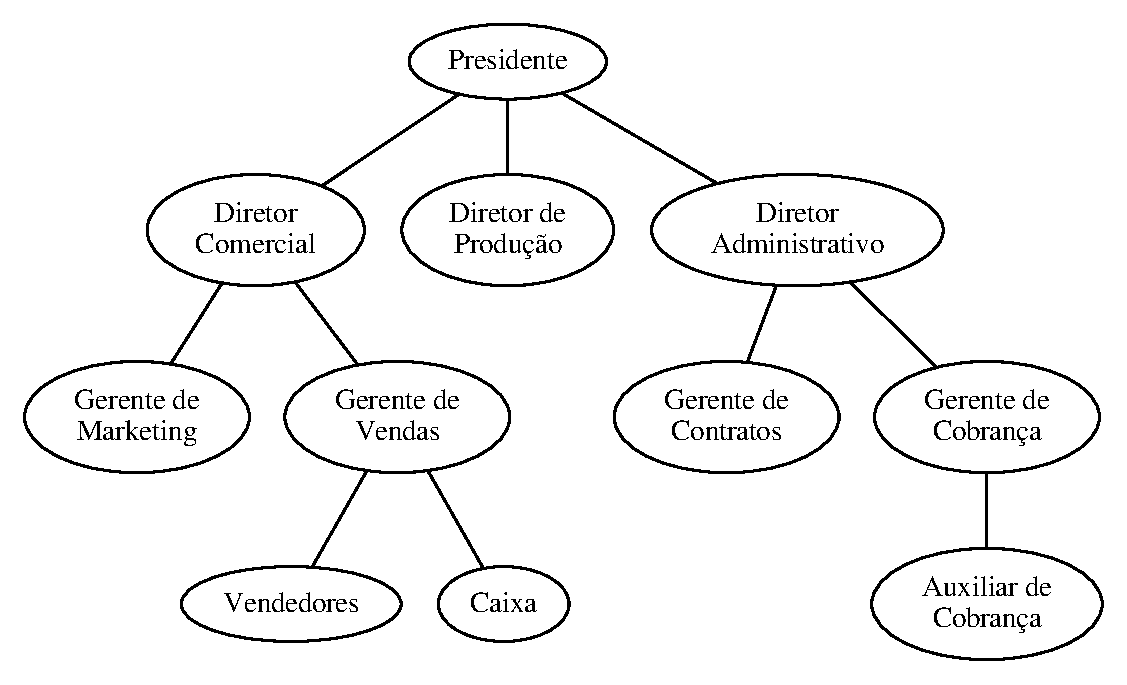
\includegraphics[height=0.55\paperheight]{imagens/arvore1.eps}
\end{figure}
\end{itemize}
\end{frame}

%-------------------------------------------------------
\begin{frame}\frametitle{Definição}
\begin{itemize}
	\item Formalmente uma árvore \textbf{T} é definida como um conjunto finito de um ou mais \textbf{nodos}, com a seguinte propriedade:
	\begin{itemize}
		\item Se \textbf{T} não é vazia, existe um nodo denominado \textbf{raiz} da árvore
		\item Os demais nodos formam $m > 0$ conjuntos disjuntos $S_1$, $S_2$, ..., $S_m$, sendo cada um destes conjuntos uma árvore
		\item As árvores $S_i$ ($1 \le i \le m$) são chamadas de \textbf{subárvores}
	\end{itemize}
	\item Pela definição
	\begin{itemize}
		\item Cada nodo da árvore é a raiz de uma subárvore
	\end{itemize}
\end{itemize}
\end{frame}

%-------------------------------------------------------
\begin{frame}\frametitle{Definição}
\begin{itemize}
	\item Portanto, uma árvore pode ser representada da seguinte forma:
\begin{figure}[h]
	\centering
	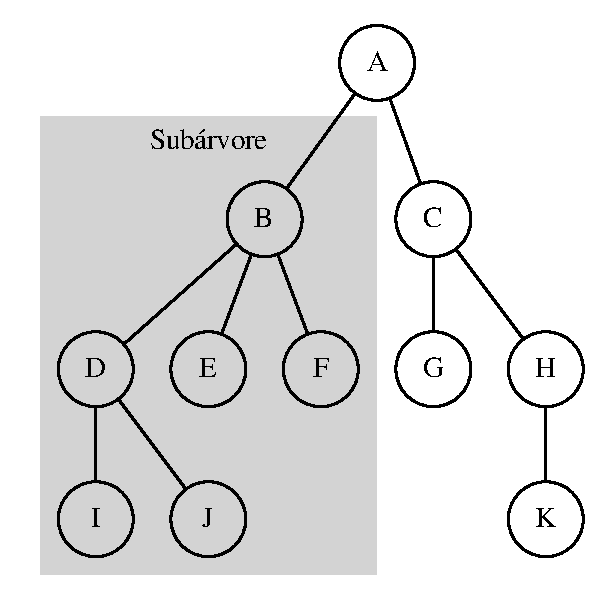
\includegraphics[height=0.60\paperheight]{imagens/arvore2.eps}
\end{figure}
	\item \textbf{A} é a raiz da árvore
\end{itemize}
\end{frame}

%-------------------------------------------------------
\begin{frame}\frametitle{Relacionamentos entre nodos	}
\begin{itemize}
	\item Outra propriedade de uma árvore \textbf{T}:
	\begin{itemize}
		\item Cada nodo \textbf{v} de \textbf{T} diferente da raiz tem um único nodo \textbf{pai}, \textbf{w}
		\item Todo nodo com \textbf{pai} \textbf{w} é \textbf{filho} de \textbf{w}
	\end{itemize}
	\item Pela definição
	\begin{itemize}
		\item Uma árvore pode ser vazia, isto é, não possui nodos
		\item Esta convenção permite que se defina uma árvore recursivamente
		\begin{itemize}
			\item Uma árvore \textbf{T} ou está vazia, ou consiste de um nodo \textbf{r}, chamado de raiz de \textbf{T}, e um conjunto de árvores cujas raízes são filhas de \textbf{r}
		\end{itemize}
	\end{itemize}
\end{itemize}
\end{frame}
	
%-------------------------------------------------------
\begin{frame}\frametitle{Relacionamentos entre nodos}
\begin{itemize}
	\item Outros relacionamentos entre nodos
	\begin{itemize}
		\item Dois nodos que são filhos de um mesmo pai são \textbf{irmãos}
		\item Um nodo \textbf{v} é \textbf{externo} se \textbf{v} não tem filhos
		\item Um nodo \textbf{v} é \textbf{interno} se tem um ou mais filhos
	\end{itemize}
	\item Nodo \textbf{interno} também é conhecido como \textbf{galho}
	\item Nodo \textbf{externo} também é conhecido como \textbf{folha}
\end{itemize}
\end{frame}

%-------------------------------------------------------
\begin{frame}\frametitle{Relacionamentos entre nodos}
\begin{itemize}
	\item A raiz de uma árvore é chamada de \textbf{pai} de suas subárvores
	\item As raízes das subárvores de um nodo são chamadas de \textbf{irmãos}, que, por sua vez, são \textbf{filhos} de seu nodo pai
\begin{columns}[T]
\begin{column}{0.5\linewidth}
%\vspace{-3mm}
\begin{figure}[h]
	\centering
	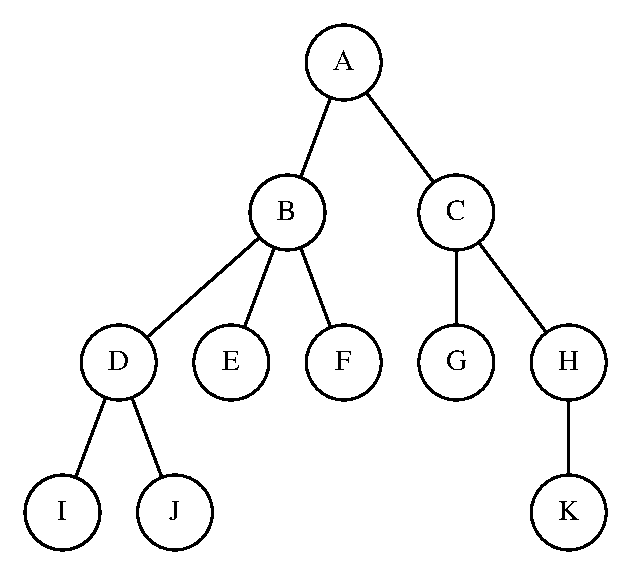
\includegraphics[height=0.55\paperheight]{imagens/arvore3.eps}
\end{figure}
\end{column}
\begin{column}{0.5\linewidth}
%\vspace{3mm}
\begin{itemize}
	\item \textbf{A} é pai de \textbf{B} e \textbf{C}
	\item \textbf{D}, \textbf{E} e \textbf{F} são irmãos
	\item \textbf{I} é filho de \textbf{J}
\end{itemize}
\end{column}
\end{columns}
\end{itemize}
\end{frame}

%-------------------------------------------------------
\begin{frame}\frametitle{``Árvore Invertida''}
\begin{figure}[h]
	\centering
	\includegraphics[height=0.60\paperheight]{imagens/arvore_invertida.png}\\
{\tiny Fonte: \url{https://di.ubi.pt/~cbarrico/Disciplinas/AlgoritmosEstruturasDadosLEI/Downloads/Teorica_ConceitosGeraisArvores.pdf}}
\end{figure}
\end{frame}

%-------------------------------------------------------
\begin{frame}\frametitle{Exemplo}
\begin{columns}[T]
\begin{column}{0.4\linewidth}
%\vspace{-3mm}
\begin{itemize}
	\item Organização hierárquica dos arquivos nos sistemas operacionais é uma árvore
	\item Nodos internos, neste caso, são associados a diretórios, e nodos externos a arquivos
	\item No Linux o diretório raiz é “/”
\end{itemize}
\end{column}
\begin{column}{0.6\linewidth}
\vspace{-5mm}
\begin{figure}[h]
	\centering
	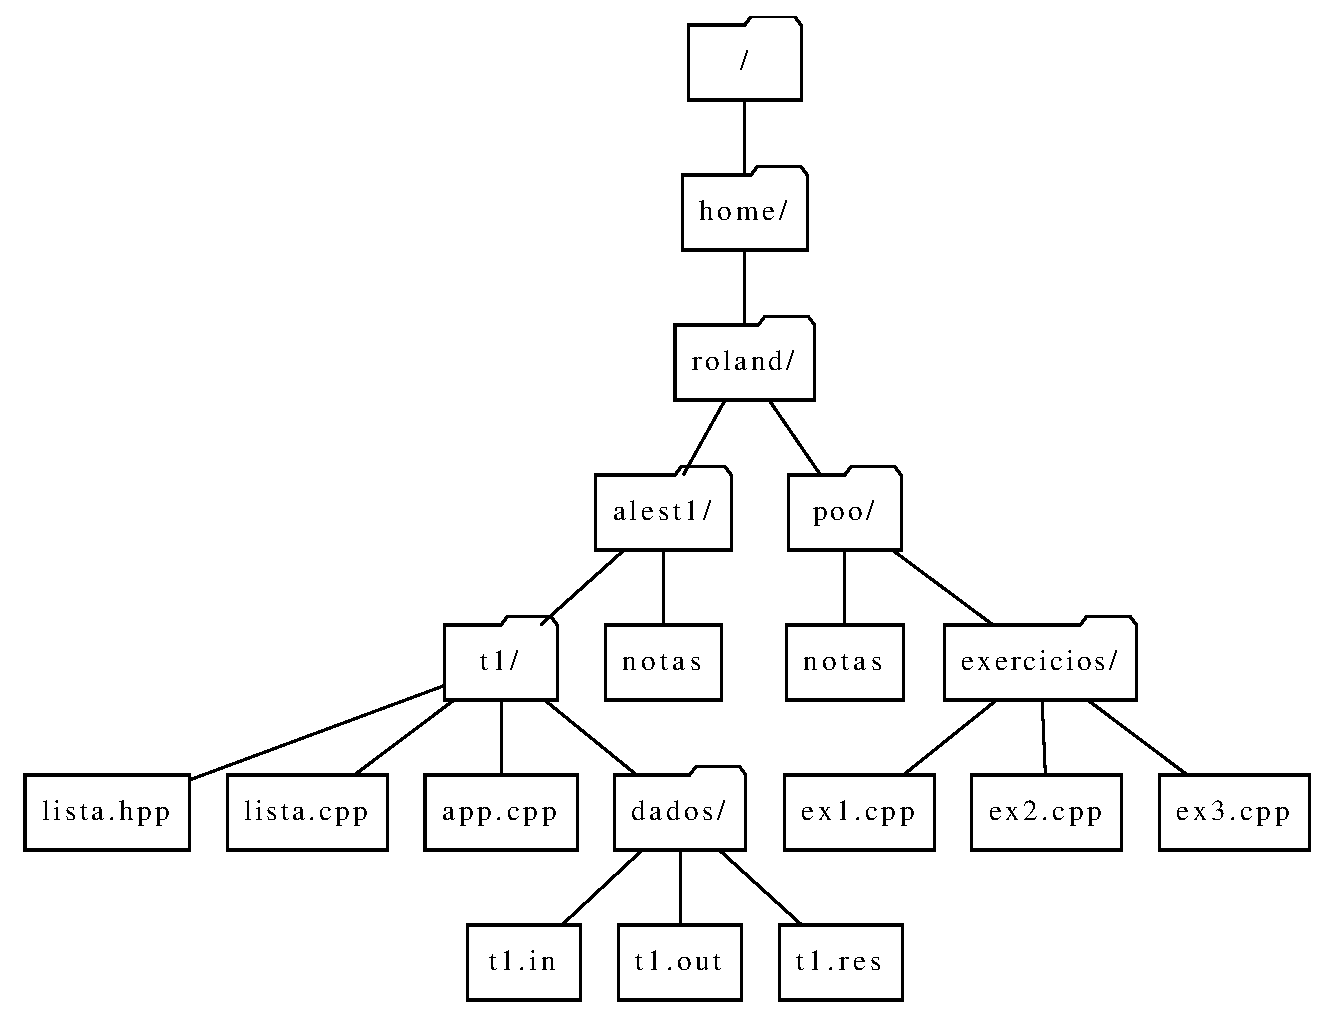
\includegraphics[height=0.7\paperheight]{imagens/arvore4.eps}
\end{figure}
\end{column}
\end{columns}
\end{frame}

%-------------------------------------------------------
\begin{frame}\frametitle{Arestas e Caminhos em Árvores}
\begin{columns}[T]
\begin{column}{0.4\linewidth}
%\vspace{-3mm}
\begin{itemize}
	\item Uma \textbf{\underline{aresta}} de uma árvore \textbf{T} é um par de nodos (\textbf{u},\textbf{v}) tal que \textbf{u} é pai de \textbf{v}, ou vice-versa
	\item Um \textbf{\underline{caminho}} de \textbf{T} é uma sequência de nodos tais que quaisquer dois nodos consecutivos
da sequência formam uma aresta
	\item Exemplo: \texttt{alest1/}, \texttt{t1/}, \texttt{dados/} e \texttt{t1.out} formam um caminho
\end{itemize}
\end{column}
\begin{column}{0.6\linewidth}
\vspace{-5mm}
\begin{figure}[h]
	\centering
	\includegraphics[height=0.7\paperheight]{imagens/arvore4-v2.eps}
\end{figure}
\end{column}
\end{columns}
\end{frame}

%-------------------------------------------------------
\begin{frame}\frametitle{Grau, Nível e Altura}
\begin{itemize}
	\item  Grau
	\begin{itemize}
		\item É o número de subárvores de um nodo
		\item Quando o grau é zero, ou seja, o nodo não possui filhos, ele é \textbf{folha}
	\end{itemize}
	\item Nível de um nodo
	\begin{itemize}
		\item É o número de linhas que liga o nodo à raiz, sabendo que a raiz é o nível zero
	\end{itemize}
	\item Altura
	\begin{itemize}
		\item É definida como sendo o nível mais alto da árvore
	\end{itemize}
\end{itemize}
\end{frame}

%-------------------------------------------------------
\begin{frame}\frametitle{Grau, Nível e Altura}
\begin{columns}[T]
\begin{column}{0.4\linewidth}
%\vspace{-3mm}
\begin{itemize}
	\item Grau:
	\begin{itemize}
		\item Nodo A:
		\item Nodo B:
		\item Nodo C:
		\item Nodo D:
		\item Nodo E:
		\item Nodo F:
		\item Nodo G:
		\item Nodo H:
		\item Nodo I:
		\item Nodo J:
		\item Nodo K:
	\end{itemize}
\end{itemize}
\end{column}
\begin{column}{0.6\linewidth}
\vspace{-5mm}
\begin{figure}[h]
	\centering
	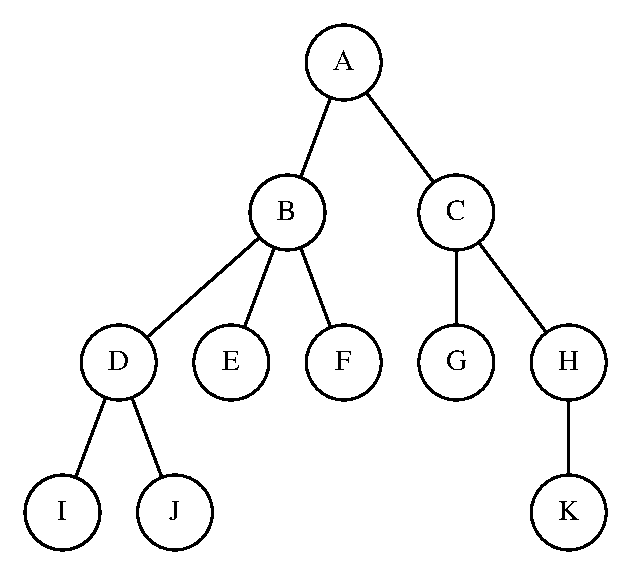
\includegraphics[height=0.70\paperheight]{imagens/arvore3.eps}
\end{figure}
\end{column}
\end{columns}
\end{frame}

%-------------------------------------------------------
\begin{frame}\frametitle{Grau, Nível e Altura}
\begin{columns}[T]
\begin{column}{0.4\linewidth}
%\vspace{-3mm}
\begin{itemize}
	\item Grau:
	\begin{itemize}
		\item Nodo A: 2
		\item Nodo B: 3
		\item Nodo C: 2
		\item Nodo D: 2
		\item Nodo E: 0
		\item Nodo F: 0
		\item Nodo G: 0
		\item Nodo H: 1
		\item Nodo I: 0
		\item Nodo J: 0
		\item Nodo K: 0
	\end{itemize}
\end{itemize}
\end{column}
\begin{column}{0.6\linewidth}
\vspace{-5mm}
\begin{figure}[h]
	\centering
	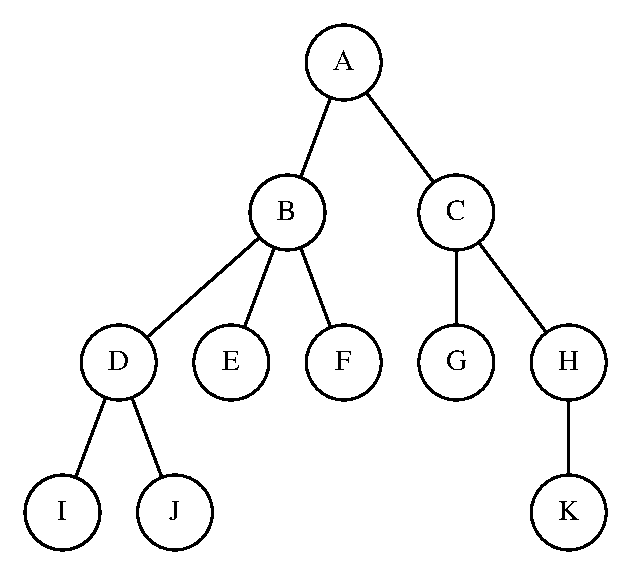
\includegraphics[height=0.70\paperheight]{imagens/arvore3.eps}
\end{figure}
\end{column}
\end{columns}
\end{frame}

%-------------------------------------------------------
\begin{frame}\frametitle{Grau, Nível e Altura}
\begin{columns}[T]
\begin{column}{0.4\linewidth}
%\vspace{-3mm}
\begin{itemize}
	\item Nível:
	\begin{itemize}
		\item Nodo A:
		\item Nodo B:
		\item Nodo C:
		\item Nodo D:
		\item Nodo E:
		\item Nodo F:
		\item Nodo G:
		\item Nodo H:
		\item Nodo I:
		\item Nodo J:
		\item Nodo K:
	\end{itemize}
	\item Altura:
	\begin{itemize}
		\item Árvore:
	\end{itemize}
\end{itemize}
\end{column}
\begin{column}{0.6\linewidth}
\vspace{-5mm}
\begin{figure}[h]
	\centering
	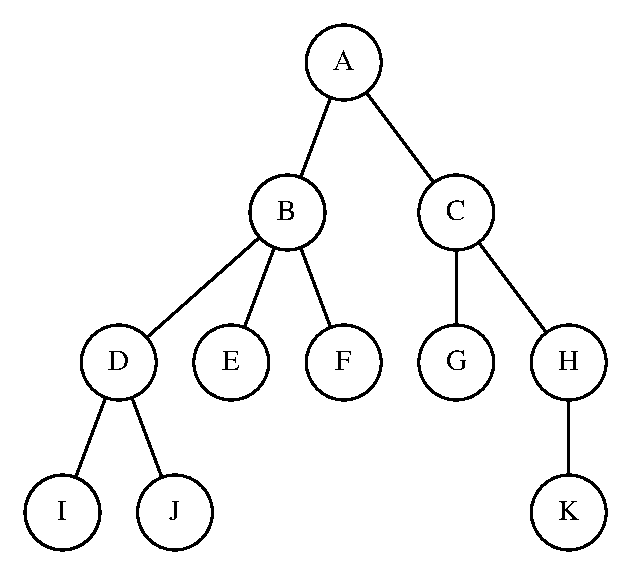
\includegraphics[height=0.70\paperheight]{imagens/arvore3.eps}
\end{figure}
\end{column}
\end{columns}
\end{frame}

%-------------------------------------------------------
\begin{frame}\frametitle{Grau, Nível e Altura}
\begin{columns}[T]
\begin{column}{0.4\linewidth}
%\vspace{-3mm}
\begin{itemize}
	\item Nível:
	\begin{itemize}
		\item Nodo A: 0
		\item Nodo B: 1
		\item Nodo C: 1
		\item Nodo D: 2
		\item Nodo E: 2
		\item Nodo F: 2
		\item Nodo G: 2
		\item Nodo H: 2
		\item Nodo I: 3
		\item Nodo J: 3
		\item Nodo K: 3
	\end{itemize}
	\item Altura:
	\begin{itemize}
		\item Árvore: 3
	\end{itemize}
\end{itemize}
\end{column}
\begin{column}{0.6\linewidth}
\vspace{-5mm}
\begin{figure}[h]
	\centering
	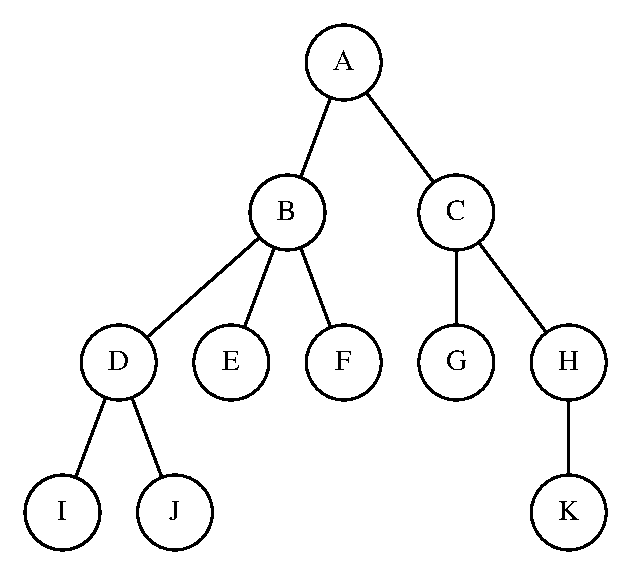
\includegraphics[height=0.70\paperheight]{imagens/arvore3.eps}
\end{figure}
\end{column}
\end{columns}
\end{frame}

%-------------------------------------------------------
\begin{frame}\frametitle{Grau, Nível e Altura}
\begin{columns}[T]
\begin{column}{0.4\linewidth}
%\vspace{-3mm}
\begin{itemize}
	\item Raiz: A
	\item Nodos internos: B, C, D, H
	\item Folhas: I, J, E, F, G, K
	\end{itemize}
\end{column}
\begin{column}{0.6\linewidth}
\vspace{-5mm}
\begin{figure}[h]
	\centering
	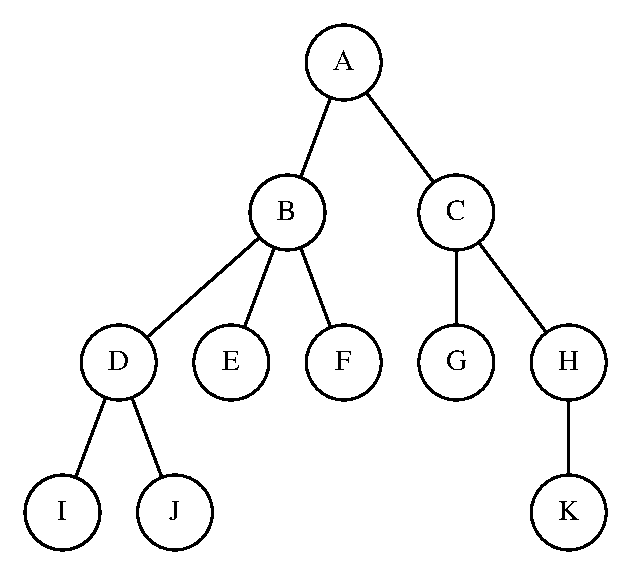
\includegraphics[height=0.70\paperheight]{imagens/arvore3.eps}
\end{figure}
\end{column}
\end{columns}
\end{frame}

%-------------------------------------------------------
\begin{frame}\frametitle{Floresta}
\begin{itemize}
	\item Conjunto de uma ou mais árvores disjuntas
	\item Se eliminarmos o nodo raiz de uma árvore, obtém-se uma floresta
	\item Os filhos da raiz original irão se transformar nas raízes das novas árvores
\end{itemize}
\begin{figure}[h]
	\centering
	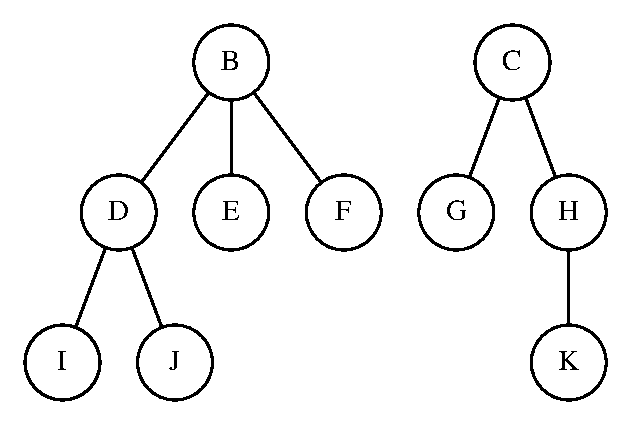
\includegraphics[height=0.5\paperheight]{imagens/floresta.eps}
\end{figure}
\end{frame}

%=======================================================
\section{Exercícios}

%-------------------------------------------------------
\begin{frame}[fragile]\frametitle{Exercício 1}
\begin{enumerate}
        \setcounter{enumi}{0}
\item Analise a árvore abaixo.
\begin{columns}[T]
\begin{column}{0.5\linewidth}
%\vspace{-5mm}
\begin{figure}[h]
	\centering
	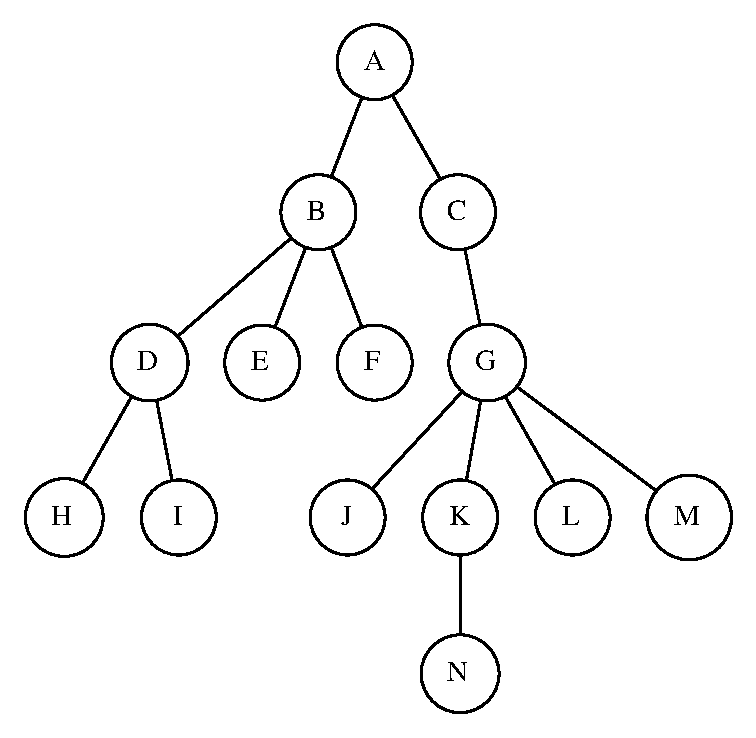
\includegraphics[height=0.6\paperheight]{imagens/exercicio01.eps}
\end{figure}
\end{column}
\begin{column}{0.5\linewidth}
E responda:
\begin{itemize}
	\item Qual é a altura da árvore?\\
	\item Quais são as folhas da árvore?\\
	\item Quais são os nodos irmãos?\\
	\item Os nodos D e G são pais de que nodos?\\
	\item Qual é o grau do nodo B?\\
	\item Qual é o grau do nodo G?\\
	\item Quais são os níveis dos nodos B, G, H, L e N?\\
\end{itemize}
\end{column}
\end{columns}
\end{enumerate}
\end{frame}

%-------------------------------------------------------
\begin{frame}[fragile]\frametitle{Exercício 2}
\begin{enumerate}
        \setcounter{enumi}{1}
\item Analise a árvore abaixo.
\begin{columns}[T]
\begin{column}{0.5\linewidth}
%\vspace{-5mm}
\begin{figure}[h]
	\centering
	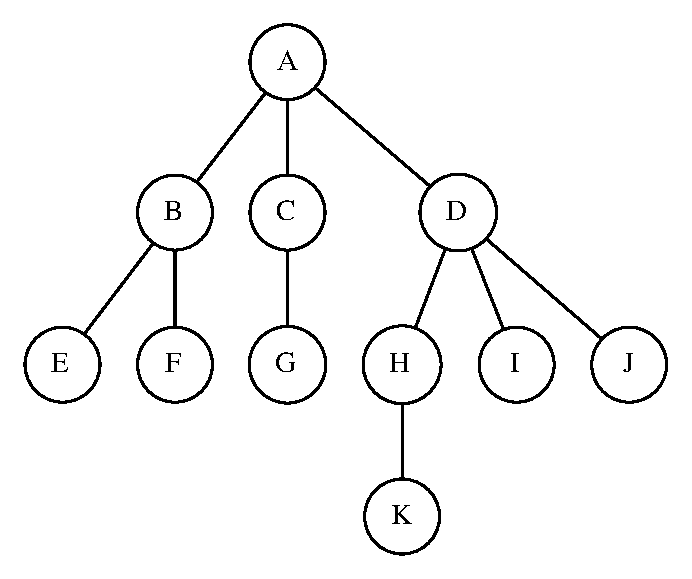
\includegraphics[height=0.5\paperheight]{imagens/exercicio02.eps}
\end{figure}
\end{column}
\begin{column}{0.5\linewidth}
E responda:
\begin{itemize}
	\item Qual é a altura da árvore?\\
	\item Quais são as folhas da árvore?\\
	\item Quais são os nodos irmãos?\\
	\item Quais são os nodos internos?
	\item Qual é o grau do nodo C?
	\item Qual é o grau do nodo D?
	\item Quais são os níveis dos nodos C, H e K?
\end{itemize}
\end{column}
\end{columns}
\end{enumerate}
\end{frame}

%=======================================================
\section{Aplicações}

%-------------------------------------------------------
\begin{frame}\frametitle{Aplicações}
\begin{itemize}
	\item Árvores são estruturas de dados adequadas para representar diversos tipos de informações
	\item Várias aplicações que podem utilizar árvores
\end{itemize}
\end{frame}

%-------------------------------------------------------
\begin{frame}\frametitle{Árvore de decisão}
\begin{itemize}
	\item Exemplo: Ir ou não ir para praia?
\begin{figure}[h]
	\centering
	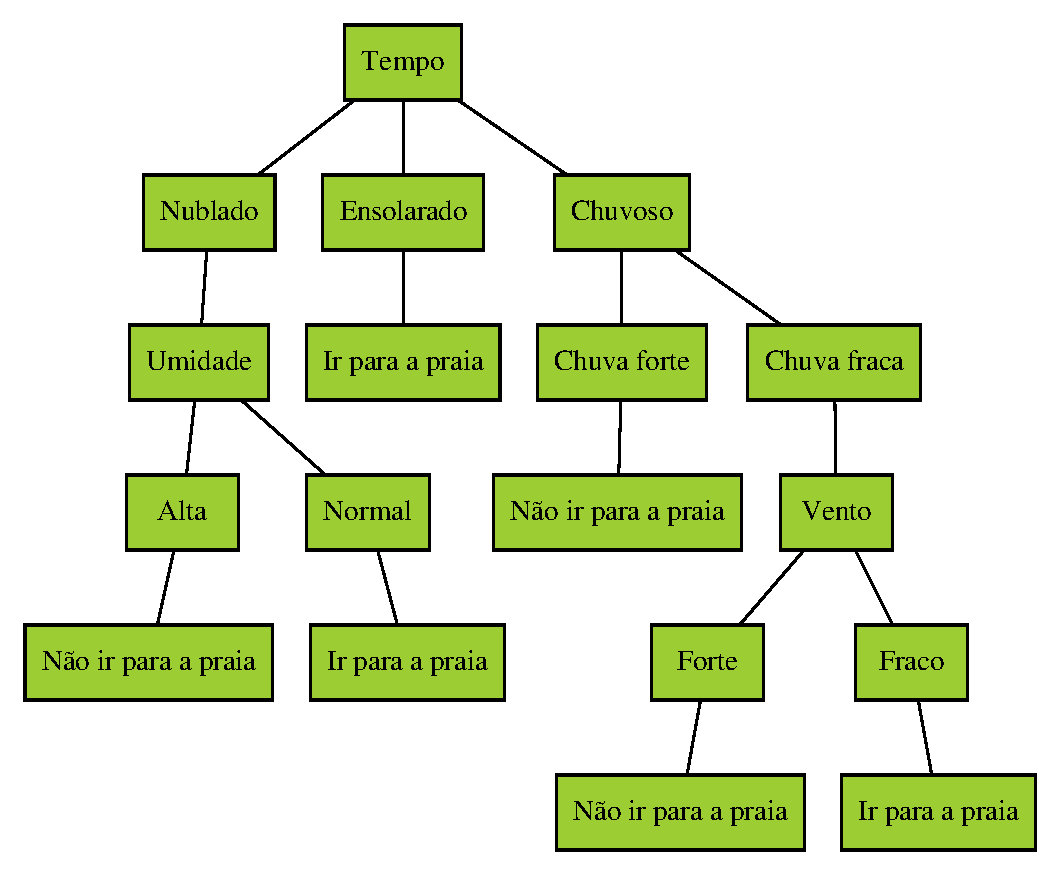
\includegraphics[height=0.65\paperheight]{imagens/arvore_de_decisao.eps}
\end{figure}
\end{itemize}
\end{frame}

%-------------------------------------------------------
\begin{frame}\frametitle{Representação de estruturas/informações hierárquicas}
\begin{itemize}
	\item Árvore genealógica
	\item Organização de livros e documentos
	\item Organização hierárquica de cargos de uma empresa
	\item Sistemas de arquivos
\begin{figure}[h]
	\centering
	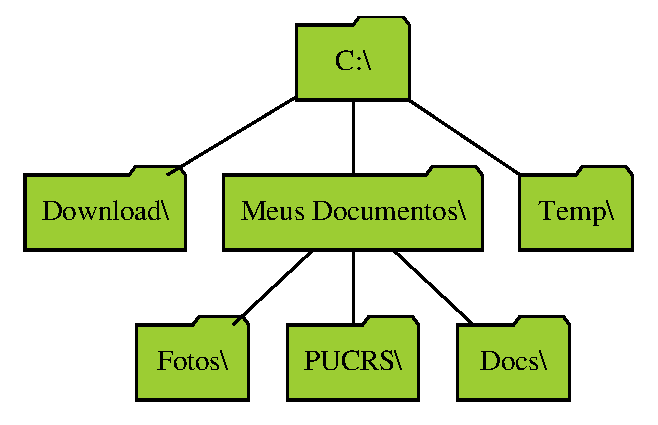
\includegraphics[height=0.4\paperheight]{imagens/arvore_de_diretorios.eps}
\end{figure}
\end{itemize}
\end{frame}

%-------------------------------------------------------
\begin{frame}[fragile]\frametitle{Representação de estruturas/informações hierárquicas}
\begin{itemize}
	\item Arquivos HTML e XML
\begin{lstlisting}[language=XML,basicstyle=\ttfamily\scriptsize]
<?xml version="1.0"?>
<Company>
  <Employee>
    <FirstName>Maria</FirstName>
    <LastName>Silva</LastName>
    <PhoneNumber>(51)98986767</PhoneNumber>
    <Email>maria.silva@gmail.com</Email>
    <Address>
      <Street>Rua dos Andradas 1586/202</Street>
      <City>Porto Alegre</City>
      <State>RS</State>
      <Zip>90021-212</Zip>
    </Address>
  </Employee>
</Company>
\end{lstlisting}
\end{itemize}
\end{frame}

%-------------------------------------------------------
\begin{frame}\frametitle{Computação Gráfica}
\begin{columns}[T]
\begin{column}{0.30\linewidth}
\begin{itemize}
	\item Grafo de cena
\end{itemize}
\begin{figure}[h]
	\centering
	\includegraphics[height=0.60\paperheight]{imagens/grafo_de_cena.png}
\end{figure}
\end{column}
\begin{column}{0.70\linewidth}
\begin{itemize}
	\item Algoritmos para remoção de superfícies escondidas (árvore \emph{Binary Space-Partitioning})
\end{itemize}
\begin{figure}[h]
	\centering
	\includegraphics[height=0.50\paperheight]{imagens/binary_space_partitioning.png}
\end{figure}
\end{column}
\end{columns}
\end{frame}

%-------------------------------------------------------
\begin{frame}\frametitle{Computação Gráfica}
\begin{itemize}
	\item Representação de objetos (Quadtree e Octree), etc.
\end{itemize}
\begin{columns}[T]
\begin{column}{0.36\linewidth}
\begin{figure}[h]
	\centering
	\includegraphics[height=0.45\paperheight]{imagens/quadtree.jpg}
\end{figure}
\end{column}
\begin{column}{0.34\linewidth}
\begin{figure}[h]
	\centering
	\includegraphics[height=0.45\paperheight]{imagens/octree.png}
\end{figure}
\end{column}
\begin{column}{0.30\linewidth}
\begin{figure}[h]
	\centering
	\includegraphics[height=0.45\paperheight]{imagens/coelho.jpg}
\end{figure}
\end{column}
\end{columns}
\end{frame}

%-------------------------------------------------------
\begin{frame}\frametitle{Eliminatórias de Campeonatos}
\begin{figure}[h]
	\centering
	\includegraphics[height=0.70\paperheight]{imagens/copa_russia_2018.jpg}
\end{figure}
\end{frame}

%-------------------------------------------------------
\begin{frame}\frametitle{Interfaces Gráficas com o Usuário}
\begin{columns}[T]
\begin{column}{0.62\linewidth}
\vspace{-5mm}
\begin{figure}[h]
	\centering
	\includegraphics[height=0.70\paperheight]{imagens/interface1.jpg}
\end{figure}
\end{column}
\begin{column}{0.38\linewidth}
\vspace{-5mm}
\begin{figure}[h]
	\centering
	\includegraphics[height=0.70\paperheight]{imagens/interface2.jpg}
\end{figure}
\end{column}
\end{columns}
\end{frame}

%-------------------------------------------------------
\begin{frame}\frametitle{Expressões Aritméticas}
\begin{itemize}
	\item Pode-se usar árvores para representar e avaliar expressões aritméticas
	\item Exemplo: \texttt{A * B + C / ( D + E )}
\begin{figure}[h]
	\centering
	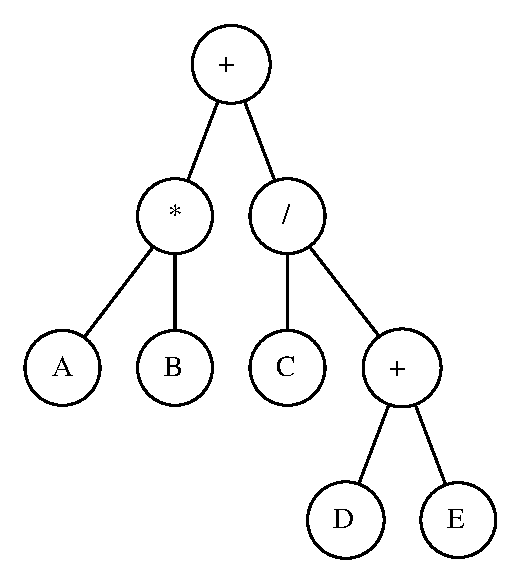
\includegraphics[height=0.6\paperheight]{imagens/expressao_aritmetica.eps}
\end{figure}
\end{itemize}
\end{frame}

%-------------------------------------------------------
\begin{frame}\frametitle{Organização das Páginas de um \emph{Site}}
\vspace{-3mm}
\begin{figure}[h]
	\centering
	\includegraphics[height=0.70\paperheight]{imagens/paginas_web.jpg}\\
{\tiny Fonte: \url{https://dribbble.com/shots/1198252-Sitemap-For-Student-Guide}}
\end{figure}	
\end{frame}

	
%=======================================================
\section{Representação na Memória}

%-------------------------------------------------------
\begin{frame}\frametitle{Representação na Memória}
\begin{itemize}
	\item Da mesma forma que as estruturas de dados lineares, podemos alocar as árvores de duas maneiras
	\begin{itemize}
		\item Por contiguidade
		\item Por encadeamento
	\end{itemize}
\end{itemize}
\end{frame}

%-------------------------------------------------------
\begin{frame}[fragile]\frametitle{Representação por Contiguidade}
\begin{itemize}
	\item A árvore é armazenada em um arranjo
	\item Cada posição por arranjo pode, por exemplo, conter, além da informação do nodo, referências aos nodos filhos
\begin{columns}[T]
\begin{column}{0.30\linewidth}
%\vspace{-5mm}
\begin{figure}[h]
	\centering
	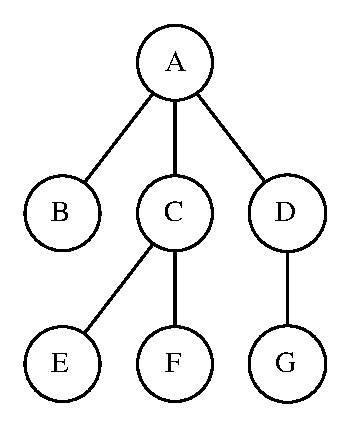
\includegraphics[height=0.4\paperheight]{imagens/arvore_a.eps}
\end{figure}
\end{column}
\begin{column}{0.70\linewidth}
\begin{figure}[h]
	\centering
	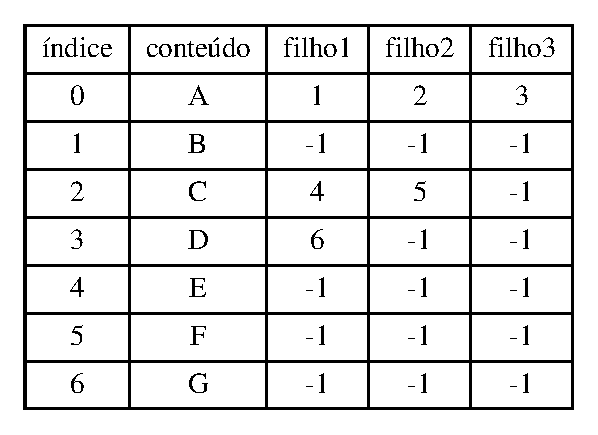
\includegraphics[height=0.4\paperheight]{imagens/arvore_a-cont.eps}
\end{figure}
\end{column}
\end{columns}
\end{itemize}
\end{frame}

%-------------------------------------------------------
\begin{frame}\frametitle{Representação por Contiguidade}
\begin{itemize}
	\item Vantagem:
	\begin{itemize}
		\item Forma de armazenar árvores em arquivos
	\end{itemize}
	\item Desvantagem:
	\begin{itemize}
		\item Quantidade de processamento para inserção, remoção ou mesmo localização de um nodo
	\end{itemize}
\end{itemize}
\end{frame}

%-------------------------------------------------------
\begin{frame}[fragile]\frametitle{Representação por Encadeamento}
\begin{itemize}
	\item Forma \textbf{mais usual}
	\item Facilita as operações de inserção, remoção e pesquisa na árvore
	\item Cada nodo conterá, além da informação, as referências das suas subárvores
\begin{columns}[T]
\begin{column}{0.30\linewidth}
%\vspace{-5mm}
\begin{figure}[h]
	\centering
	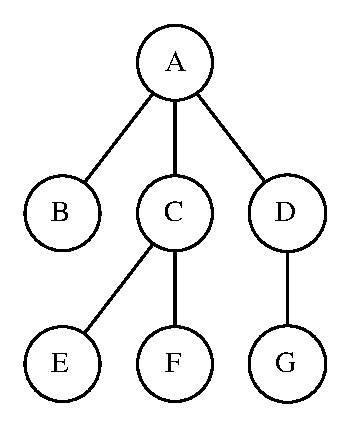
\includegraphics[height=0.4\paperheight]{imagens/arvore_a.eps}
\end{figure}
\end{column}
\begin{column}{0.70\linewidth}
\begin{figure}[h]
	\centering
	\includegraphics[height=0.35\paperheight]{imagens/arvore_a-enc.png}
\end{figure}
\end{column}
\end{columns}
\end{itemize}
\end{frame}

%-------------------------------------------------------
\begin{frame}\frametitle{Representação por Encadeamento}
\begin{itemize}
	\item  No caso de árvores ``genéricas'', cada nodo pode ter uma quantidade de subárvores diferentes
	\item Torna-se necessário:
	\begin{itemize}
		\item Limitar, ou seja, determinar o número máximo de subárvores que cada nodo deve conter
		\item Ou ter uma lista de subárvores
	\end{itemize}
	\item Isso é necessário, pois os nodos de uma mesma árvore são todos do mesmo tipo
\end{itemize}
\end{frame}

%-------------------------------------------------------
\begin{frame}\frametitle{Exemplo}
\begin{columns}[T]
\begin{column}{0.25\linewidth}
%\vspace{-5mm}
\begin{figure}[h]
	\centering
	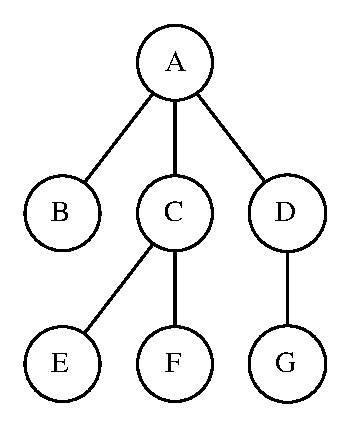
\includegraphics[height=0.4\paperheight]{imagens/arvore_a.eps}
\end{figure}
\end{column}
\begin{column}{0.75\linewidth}
\pause\lstinputlisting[basicstyle=\ttfamily\tiny]{src/exemplo01.cpp}
\end{column}
\end{columns}
\end{frame}

%-------------------------------------------------------
\begin{frame}\frametitle{GraphViz}
\vspace{-2mm}
\begin{figure}[h]
	\centering
	\includegraphics[height=0.25\paperheight]{imagens/graphviz.png}
\end{figure}
\vspace{-3mm}
\begin{itemize}
	\item Graphviz (abreviação de \emph{Graph Visualization Software}) é uma ferramenta de código-fonte aberto para desenhar grafos (formados por nodos e arestas) especificados a partir de uma linguagem de escrite chamada DOT (que usa a extensão ``gv'')
	\item GraphViz também provê bibliotecas para que aplicações possam usar suas facilidades
	\item É um \emph{software} livre licenciado através da Licença Pública Eclipse
	\item Página: \url{https://graphviz.org/}
	\item Há várias opções para gerar imagens a partir dos arquivos no formato DOT
	\begin{itemize}
		\item \url{https://dreampuf.github.io/GraphvizOnline/}
	\end{itemize}
\end{itemize}
\end{frame}

%-------------------------------------------------------
\begin{frame}[fragile]\frametitle{GraphViz}
\begin{columns}[T]
\begin{column}{0.3\linewidth}
%\vspace{-5mm}
\textbf{\underline{Grafo:}}\\
\begin{figure}[h]
	\centering
	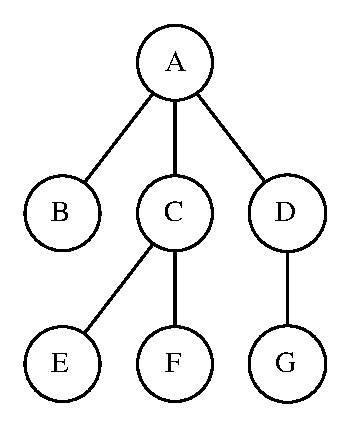
\includegraphics[height=0.4\paperheight]{imagens/arvore_a.eps}
\end{figure}
\end{column}
\begin{column}{0.35\linewidth}
\textbf{\underline{Versão 1:}}\\
\lstinputlisting[basicstyle=\ttfamily\tiny]{imagens/arvore_a.gv}
\end{column}
\begin{column}{0.35\linewidth}
\textbf{\underline{Versão 2:}}\\
\lstinputlisting[basicstyle=\ttfamily\tiny]{imagens/arvore_a-v2.gv}
\end{column}
\end{columns}
\end{frame}

%=======================================================
\section{Exercícios}

%-------------------------------------------------------
\begin{frame}[fragile]\frametitle{Exercício 3}
\begin{enumerate}
        \setcounter{enumi}{2}
	\small
	\item Considere a árvore e o programa que cria esta árvore correspondente, usando estruturas encadeadas em C++, ambos apresentados na próxima página. Observe que o nodo declarado (\texttt{struct Node}) armazena um caractere (\texttt{char}) e suporta até 3 subárvores (ou seja, cada nodo pode ter 3 nodos filhos). Para este programa, implemente as seguintes funções:
	\begin{itemize}
		\footnotesize
		\item \texttt{void clean(Node *root)}: que recebe o endereço de um nodo e faz a desalocação de todos os nodos da árvore a partir do nodo recebido (\texttt{root}) -- esta função deve ser implementada de forma recursiva;
		\item \texttt{string strGraphViz(Node *root)}: que recebe o endereço de um nodo e gera uma cadeia de caracteres (\texttt{string}) com representação da árvore no formato DOT, usado pelo GraphViz -- esta função deve: imprimir a parte inicial do formato DOT; chamar um outro método recursivo (por exemplo, \texttt{string strNode(Node *node)}) para gerar a lista de arestas entre os nodos; imprimir a parte final do formato DOT.
	\end{itemize}
	Rode o seu programa, por exemplo, com:
\begin{lstlisting}[basicstyle=\ttfamily\scriptsize,language=bash]
./exercicio03 > exercicio03.gv
\end{lstlisting}
	Use o site \url{https://dreampuf.github.io/GraphvizOnline/} para verificar se o arquivo \texttt{exercicio03.gv} foi corretamente gerado.
\end{enumerate}
\end{frame}

%-------------------------------------------------------
\begin{frame}[fragile]\frametitle{Exercício 3}
\begin{columns}
\begin{column}{0.23\linewidth}
%\vspace{-5mm}
\begin{figure}[h]
	\centering
	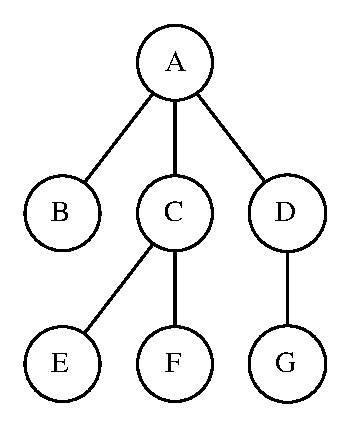
\includegraphics[height=0.4\paperheight]{imagens/arvore_a.eps}
\end{figure}
\end{column}
\begin{column}{0.77\linewidth}
\fontsize{6pt}{6pt}\selectfont{
\lstinputlisting{src/exercicio03.cpp}
}
\end{column}
\end{columns}
\end{frame}

%-------------------------------------------------------
\begin{frame}[fragile]\frametitle{Exercício 4}
\begin{enumerate}
        \setcounter{enumi}{3}
	\small
	\item Considere a árvore abaixo e, usando como modelo o código do exercício 3 (resolvido), implemente um programa em C++ que crie esta árvore em memória, que a imprima no formato DOT e que desaloque corretamente todos os nodos da árvore. Use o site \url{https://dreampuf.github.io/GraphvizOnline/} para verificar se o arquivo DOT foi corretamente gerado.
\begin{figure}[h]
	\centering
	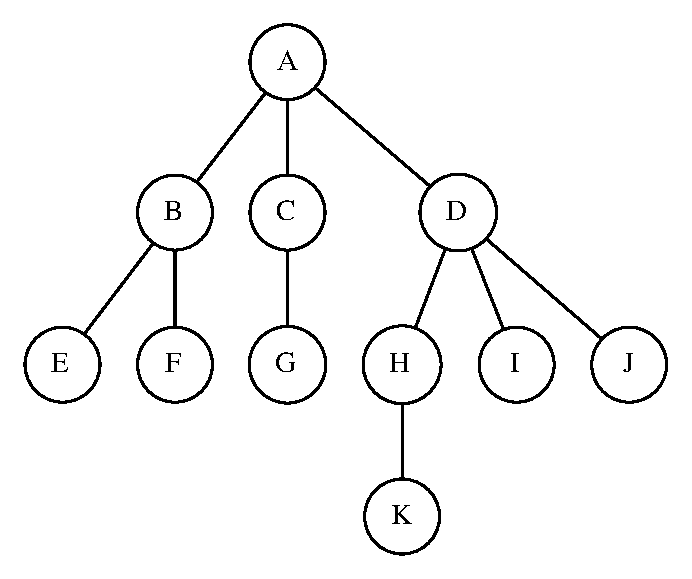
\includegraphics[height=0.5\paperheight]{imagens/exercicio02.eps}
\end{figure}
\end{enumerate}
\end{frame}

%=======================================================
\section{TAD para Árvore}

%-------------------------------------------------------
\begin{frame}\frametitle{TAD para Árvore}
\begin{itemize}
	\item Um TAD para árvore:
	\begin{itemize}
		\item Armazena elementos em nodos
		\item O posicionamento dos nodos satisfaz as relações pai-filho
		\item Operações consideram as propriedades desta estrutura de dados hierárquica
	\end{itemize}
\end{itemize}
\end{frame}

%-------------------------------------------------------
\begin{frame}\frametitle{TAD para Árvore}
\begin{itemize}
	\item Uma árvore deve disponibilizar métodos de acesso que retornam e aceitam posições:
	\begin{itemize}
		\item \texttt{root()}: retorna a raiz da árvore
		\item \texttt{parent(v)}: retorna o nodo pai de \texttt{v}, ocorrendo um erro se for a raiz
		\item \texttt{children(v)}: retorna os filhos do nodo \texttt{v}
	\end{itemize}
\end{itemize}
\end{frame}

%-------------------------------------------------------
\begin{frame}\frametitle{TAD para Árvore}
\begin{itemize}
	\item Métodos de consulta:
	\begin{itemize}
		\item \texttt{isInternal(v)}: testa se um nodo \texttt{v} é interno e retorna \texttt{true} ou \texttt{false}
		\item \texttt{isExternal(v)}: testa se um nodo \texttt{v} é externo e retorna \texttt{true} ou \texttt{false}
		\item \texttt{isRoot(v)}: testa se um nodo \texttt{v} é raiz e retorna \texttt{true} ou \texttt{false}
	\end{itemize}
\end{itemize}
\end{frame}

%-------------------------------------------------------
\begin{frame}\frametitle{TAD para Árvore}
\begin{itemize}
	\item Métodos ``genéricos'' (não estão necessariamente relacionados com sua estrutura):
	\begin{itemize}
		\item \texttt{size()}: retorna o número de nodos na árvore
		\item \texttt{isEmpty()}: testa se a árvore tem ou não tem algum nodo
		\item \texttt{iterator()}: retorna um iterator de todos os elementos armazenados nos nodos da árvore
		\item \texttt{positions()}: retorna uma coleção com todos os nodos da árvore
		\item \texttt{replaceElement(v,e)}: retorna o elemento armazenado em \texttt{v} e o substitui por \texttt{e}
	\end{itemize}
\end{itemize}
\end{frame}

%=======================================================
\section{Observação}

%-------------------------------------------------------
\begin{frame}[fragile]\frametitle{Sobre a Solução dos Exercícios 3 e 4}
\begin{itemize}
	\item Os exercícios 3 e 4 usam o método recursivo \texttt{clean()} para desalocar árvores
\begin{lstlisting}[language=C++,basicstyle=\ttfamily\tiny]
void clean(Node *subtree) {
  if ( subtree->child1 != nullptr ) clean(subtree->child1);
  if ( subtree->child2 != nullptr ) clean(subtree->child2);
  if ( subtree->child3 != nullptr ) clean(subtree->child3);
  delete subtree;
}
\end{lstlisting}
	\item Considerando-se que \texttt{root} é um \texttt{Node *} e é a raiz da árvore, a sua desalocação seria então feita usando-se \texttt{clean(root);}
\item Uma alternativa mais interessante poderia ser usar o método destrutor para isso:
\begin{lstlisting}[language=C++,basicstyle=\ttfamily\tiny]
~Node() {
  if ( child1 != nullptr ) delete child1;
  if ( child2 != nullptr ) delete child2;
  if ( child3 != nullptr ) delete child3;
  cerr << "- Node("<< info << ") destruido..." << endl;
}
\end{lstlisting}
	\item Neste caso a árvore seria desalocada usando-se \texttt{delete root;}
\end{itemize}
\end{frame}

%=======================================================
\section{Árvore Binária}

%-------------------------------------------------------
\begin{frame}[fragile]\frametitle{Árvore Binária}
\begin{itemize}
	\item Uma árvore binária é aquela na qual o grau de cada nodo é menor ou igual a 2
	\item As subárvores de um nodo são chamadas de
	\begin{itemize}
		\item Subárvore da esquerda
		\item Subárvore da direita
	\end{itemize}
\begin{figure}[h]
	\centering
	\includegraphics[height=0.5\paperheight]{imagens/arvore_binaria1-v2.eps}
\end{figure}
\end{itemize}
\end{frame}

%-------------------------------------------------------
\begin{frame}[fragile]\frametitle{Árvore Binária}
\begin{itemize}
	\item Se o grau de um nodo é 1, deve-se especificar se a sua subárvore é a da esquerda ou a da direita
\begin{figure}[h]
	\centering
	\includegraphics[height=0.35\paperheight]{imagens/arvores_binarias_diferentes.eps}
\end{figure}
\end{itemize}
\end{frame}

%-------------------------------------------------------
\begin{frame}[fragile]\frametitle{Árvore Binária Própria}
\begin{itemize}
	\item Uma árvore binária é \textbf{própria} se cada um de seus nodos internos tiver dois filhos
	\item Todos os nodos, com exceção dos nodos-folha, têm exatamente dois filhos
\begin{figure}[h]
	\centering
	\includegraphics[height=0.5\paperheight]{imagens/arvore_binaria2.eps}
\end{figure}
\end{itemize}
\end{frame}

%-------------------------------------------------------
\begin{frame}[fragile]\frametitle{Árvores de Decisão}
\begin{itemize}
	\item Classe importante de árvores binárias
	\item Quando se quer representar as diferentes saídas que podem resultar a partir das respostas a um conjunto de perguntas do tipo sim ou não
	\item Cada nodo interno é associado com uma questão
\begin{figure}[h]
	\centering
	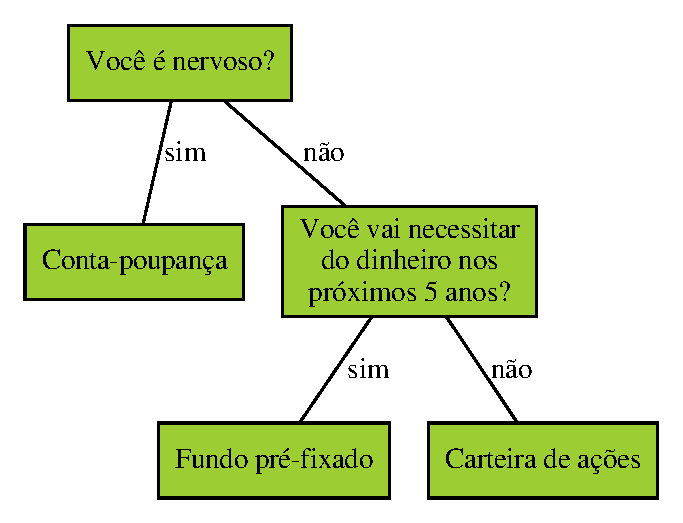
\includegraphics[height=0.5\paperheight]{imagens/arvore_de_decisao2.eps}
\end{figure}
\end{itemize}
\end{frame}

%-------------------------------------------------------
\begin{frame}\frametitle{Árvore Binária}
\begin{itemize}
	\item  Os nodos de uma árvore binária terão no mínimo:
	\begin{itemize}
		\item A informação
		\item Referência para o nodo da esquerda
		\item Referência para o nodo da direita
	\end{itemize}
	\item Também se pode usar referência para o nodo pai (o que facilita a ``navegação'')
	\item Árvores binárias são fáceis de implementar, pois cada nodo tem no máximo 2 filhos	
\end{itemize}
\end{frame}

%-------------------------------------------------------
\begin{frame}\frametitle{Árvore Binária}
\begin{columns}[T]
\begin{column}{0.2\linewidth}
%\vspace{-3mm}
\begin{figure}[h]
	\centering
	\includegraphics[height=0.70\paperheight]{imagens/arvore_binaria3.eps}
\end{figure}
\end{column}
\begin{column}{0.8\linewidth}
\vspace{-2mm}
\begin{figure}[h]
	\centering
	\textbf{\underline{SEM referência para o nodo-pai:}}\\	
	\includegraphics[height=0.3\paperheight]{imagens/arvore_binaria3-enc1.png}\\
	\textbf{\underline{COM referência para o nodo-pai:}}\\	
	\includegraphics[height=0.27\paperheight]{imagens/arvore_binaria3-enc2.png}
\end{figure}
\end{column}
\end{columns}
\end{frame}

%-------------------------------------------------------
\begin{frame}\frametitle{Árvore Binária}
\begin{columns}[T]
\begin{column}{0.75\linewidth}
%\vspace{-3mm}
\begin{itemize}
	\item Uma árvore qualquer pode ser transformada em árvore binária\\
	\item Passos para a transformação:\\
	\begin{enumerate}
		\item Ligar os nodos irmãos
		\item Desligar a ligação do nodo pai com os filhos, exceto o primeiro filho
	\end{enumerate}
	\item Nodos de mesmo nível (irmãos) são encadeados à direita e nodos com nível maior (filhos) são encadeados à esquerda (iniciando pelo primeiro filho)
\end{itemize}
\vspace{-4mm}
\begin{figure}[h]
	\includegraphics[height=0.3\paperheight]{imagens/arvore_b.eps} \hspace{25mm}
	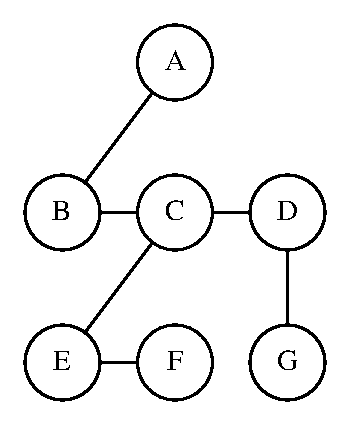
\includegraphics[height=0.3\paperheight]{imagens/arvore_b-v2.eps}
\end{figure}
\end{column}
\begin{column}{0.25\linewidth}
%\vspace{-2mm}
\begin{figure}[h]
	\centering
	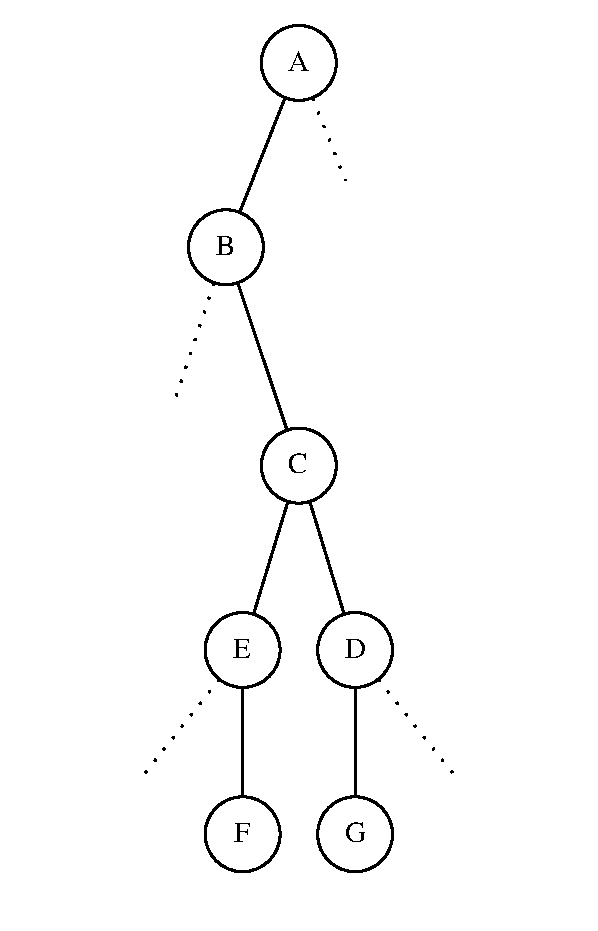
\includegraphics[height=0.7\paperheight]{imagens/arvore_b-v3.eps}
\end{figure}
\end{column}
\end{columns}
\end{frame}

%=======================================================
\section{Exercício}

%-------------------------------------------------------
\begin{frame}[fragile]\frametitle{Exercício 5}
\begin{columns}[T]
\begin{column}{0.75\linewidth}
\begin{enumerate}
        \setcounter{enumi}{4}
	\scriptsize
	\item O código apresentado nas duas páginas seguintes (\texttt{exercicio05.cpp}), define um nodo (\texttt{struct Node}) para uma árvore binária. Este nodo armazena: a informação (\texttt{info}, um único caractere), uma referência para o nodo pai (\texttt{parent}) e referências para as subárvores da esquerda (\texttt{left}) e direita (\texttt{right}). Além destas informações, o nodo contém um construtor e um destrutor. Juntamente com a definição do nodo são fornecidas funções para mostrar a árvore no formato GraphViz e uma função \texttt{main()}, que cria a árvore ao lado (usando o código fornecido) e realiza alguns testes com as funções que você deverá implementar.\\
	As funções que você deverá implementar são as seguintes:
	\begin{itemize}
		\tiny
		\item \texttt{int degree(Node *subtree)}: retorna o número de filhos (grau) de determinado nodo da árvore (parâmetro \texttt{subtree});
		\item \texttt{int depth(Node *subtree)}: retorna o nível de determinado nodo (parâmetro \texttt{subtree}) dentro da árvore (o que pode ser feito navegando pela árvore usando as referências para o nodos-pai, e contando o número de nodos até alcançar a raiz);
		\item \texttt{int size(Node *subtree)}: retorna o número de nodos que há na árvore a partir de determinado nodo (parâmetro \texttt{subtree}) -- deve ser implementado como uma função recursiva;
		\item \texttt{int treeDepth(Node *subtree)}: retorna o altura da árvore/subárvore a partir de um nodo específico (parâmetro \texttt{subtree}) -- deve ser implementado como uma função recursiva.
	\end{itemize}
Observação: os códigos usados neste exercício foram adaptados das soluções dos exercícios 3 e 4. As soluções, por outro lado, precisam ser desenvolvidas.
\end{enumerate}
\end{column}
\begin{column}{0.25\linewidth}
\begin{figure}[h]
	\centering
	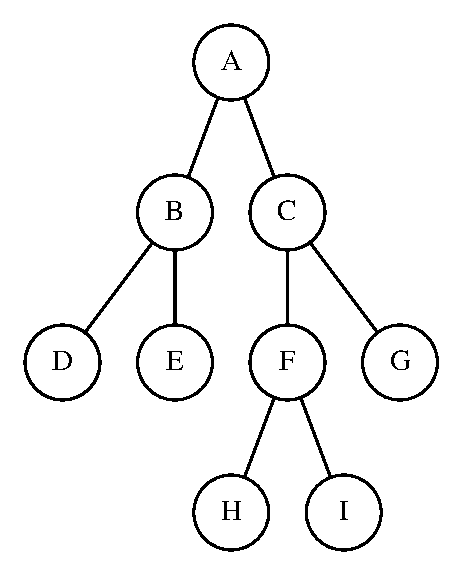
\includegraphics[height=0.4\paperheight]{imagens/exercicio05.eps}
\end{figure}
\end{column}
\end{columns}
\end{frame}

%-------------------------------------------------------
\begin{frame}[fragile]\frametitle{Exercício 5 (continuação)}
\fontsize{3pt}{5pt}\selectfont{
\lstinputlisting[firstline=1,lastline=36]{src/exercicio05.cpp}
}
\end{frame}

%-------------------------------------------------------
\begin{frame}[fragile]\frametitle{Exercício 5 (continuação)}
\fontsize{6pt}{6pt}\selectfont{
\lstinputlisting[firstline=38]{src/exercicio05.cpp}
}
\end{frame}

%=======================================================
\section{Observações}

%-------------------------------------------------------
\begin{frame}[fragile]\frametitle{Sobre a Implementação do Construtor do Exercício 5}
\begin{itemize}
	\item Observe o código que foi usado no construtor da \texttt{struct Node} do exercício 5:
\begin{lstlisting}[language=C++,basicstyle=\ttfamily\tiny]
Node(char i, Node *l = nullptr, Node *r = nullptr) {
  info = i;  left = l;  right = r;  parent = nullptr;
  if ( left != nullptr ) left->parent = this;
  if ( right != nullptr ) right->parent = this;
}
\end{lstlisting}
	\item Quando um nodo é criado, o construtor recebe as subárvores que serão inseridas como seus ``filhos''
	\item Como em cada nodo há uma referência para o nodo pai, este campo precisa ser atualizado nos nodos/subárvores filhos, o que é feito nas duas últimas linhas do construtor
	\item Para referenciar que os campos pai (\texttt{parent}) dos filhos (\texttt{left} e \texttt{right}) apontarão para o nodo que está sendo inicializado usa-se a autorreferência \texttt{\textbf{this}}
\end{itemize}
\end{frame}

%-------------------------------------------------------
\begin{frame}[fragile]\frametitle{Sobre a Solução do Exercício 5}
\begin{itemize}
	\item A solução do exercício 5 apresenta uma solução para o método \texttt{size()}, a princípio, mais fácil de entender:
\begin{lstlisting}[language=C++,basicstyle=\ttfamily\tiny]
int size(Node *subtree) {
  if (subtree == nullptr) return 0; // Somente pode ocorrer na primeira chamada,
  int res = 1;                      // ou seja, se a árvore estiver vazia
  if ( subtree->left != nullptr ) res += size(subtree->left);
  if ( subtree->right != nullptr ) res += size(subtree->right);
  return res;
}
\end{lstlisting}
	\item Veja uma solução alternativa e equivalente abaixo:
\begin{lstlisting}[language=C++,basicstyle=\ttfamily\tiny]
int size(Node *subtree) {
  if (subtree == nullptr) return 0;
  return 1 + size(subtree->left) + size(subtree->right);
}
\end{lstlisting}
	\item Analise as diferenças!
\end{itemize}
\end{frame}

%=======================================================
\section{Árvores Genéricas}

%-------------------------------------------------------
\begin{frame}\frametitle{Definição}
\begin{itemize}
	\item Formalmente uma árvore \textbf{T} é definida como um conjunto de \textbf{nodos}, que armazenam elementos em relacionamentos \textbf{pai-filho} com as seguintes propriedades:
	\begin{itemize}
		\item Se \textbf{T} não é vazia, ela tem um nodo especial chamado de \textbf{raiz} de \textbf{T} que não tem pai
		\item Cada nodo \textbf{v} de \textbf{T} diferente da raiz tem um único nodo \textbf{pai}, \textbf{w}; todo nodo com pai \textbf{w} é \textbf{filho} de \textbf{w}
	\end{itemize}
\end{itemize}
\end{frame}

%-------------------------------------------------------
\begin{frame}[fragile]\frametitle{Representações}
\begin{itemize}
	\item Textual
\begin{lstlisting}[basicstyle=\ttfamily\scriptsize]
T={A,{B,{D,{I},{J}},{E},{F}},{C,{G},{H,{K}}}}
\end{lstlisting}
\end{itemize}
\begin{columns}[T]
\begin{column}{0.5\linewidth}
%\vspace{-5mm}
\begin{itemize}
	\item GraphViz
	\lstinputlisting[basicstyle=\ttfamily\scriptsize]{imagens/arvore3.gv}
\end{itemize}
\end{column}
\begin{column}{0.5\linewidth}
\begin{itemize}
	\item Visual/Gráfica
\begin{figure}[h]
	\centering
	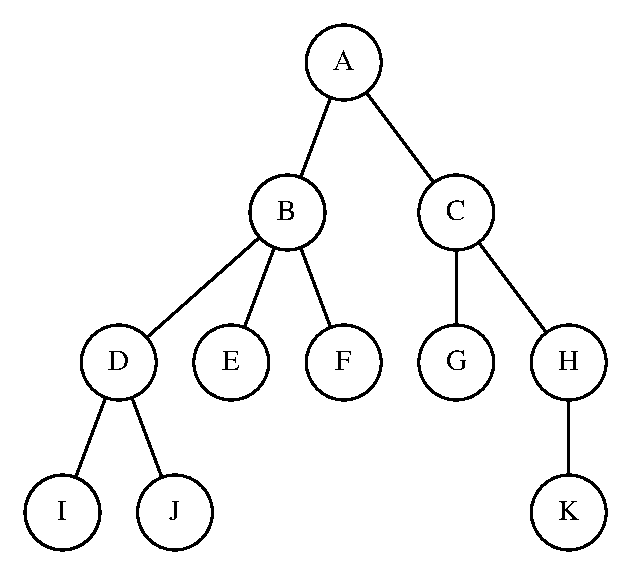
\includegraphics[height=0.4\paperheight]{imagens/arvore3.eps}
\end{figure}
\end{itemize}
\end{column}
\end{columns}
\end{frame}

%-------------------------------------------------------
\begin{frame}\frametitle{Operações}
\begin{itemize}
	\item Inserir um nodo raiz
	\item Obter o valor da raiz (da árvore e de qualquer subárvore)
	\item Esvaziar uma árvore
	\item Obter uma subárvore de um determinado nodo
	\item Anexar uma subárvore em um determinado nodo
	\item Contar o número de nodos da árvore
	\item Calcular o grau e o nível de um determinado nodo
	\item Calcular a altura de uma árvore
	\item Percorrer a árvore
	\item etc.
\end{itemize}
\end{frame}

%-------------------------------------------------------
\begin{frame}\frametitle{TAD para Árvores Genéricas}
\begin{itemize}
	\item Forma mais usual de implementação:
	\begin{itemize}
		\item Estruturas encadeadas (alocação dinâmica)
		\item Cada nodo contém:
		\begin{itemize}
			\item A informação
			\item Uma referência para o nodo pai
			\item Uma lista de referências para os nodos filhos (subárvores)
		\end{itemize}
	\end{itemize}
	\item É possível declarar um TAD para:
	\begin{itemize}
		\item O \textbf{nodo} e deixar o gerenciamento da árvore a cargo da aplicação (é necessário fornecer chamadas para acrescentar nodos filho em determinado nodo, e também para remover nodos filhos)
		\item A \textbf{estrutura de dados}, que terá uma classe interna para o nodo, determinando automaticamente onde cada informação será inserida (chamadas para acrescentar e remover algum dado NÃO precisam especificar onde a informação será inserida; nodos e referências que formam a árvore permanecem encapsulados)
	\end{itemize}
\end{itemize}
\end{frame}

%-------------------------------------------------------
\begin{frame}[fragile]\frametitle{Lista de Referências para os Nodos Filhos}
\begin{itemize}
	\item Como um nodo pode ter número variável de filhos, é interessante trabalhar com uma lista dinamicamente expansível
	\item Para implemenar esta lista dinamicamente expansível é possível usar o \emph{container} \texttt{vector} da \emph{Standard Template Library} da linguagem C++
	\item Exemplo de uso de \texttt{vector}:
\begin{lstlisting}[language=C++,basicstyle=\ttfamily\tiny]
#include <vector>

// ...

vector<int> v;   // Cria um vetor de inteiros vazio
v.push_back(10); // Adiciona 10 no vetor -> v = { 10 }
v.push_back(20); // Adiciona 20 no vetor -> v = { 10, 20 }
v.push_back(30); // Adiciona 30 no vetor -> v = { 10, 20, 30 }
v.push_back(40); // Adiciona 40 no vetor -> v = { 10, 20, 30, 40 }
v.erase( v.begin() + 1 );  // Remove o elemento de índice 1 do vetor -> v = { 10, 30, 40 }
v.pop_back();              // Remove o último elemento do vetor -> v = { 10, 30 }
for (int i=0; i<v.size(); ++i) // mostra o vetor
    cout << v[i] << endl;      // v é usado como se fosse um arranjo
\end{lstlisting}
\end{itemize}
\end{frame}

%-------------------------------------------------------
\begin{frame}[fragile]\frametitle{Declaração de um TAD de Árvore Genérica}
\fontsize{3pt}{5pt}\selectfont{
\lstinputlisting{src/NodeCharTree1/NodeCharTree.hpp}
}
\end{frame}

%-------------------------------------------------------
\begin{frame}[fragile]\frametitle{Representações}
\begin{columns}[T]
\begin{column}{0.5\linewidth}
\begin{figure}[h]
	\centering
	\includegraphics[height=0.4\paperheight]{imagens/arvore_c.eps}
\end{figure}
\end{column}
\begin{column}{0.5\linewidth}
...
\end{column}
\end{columns}
\end{frame}


\begin{comment}
// Atributos
Node father
Integer element
LinkedListOfNodes subtrees
// Métodos
Node (Integer element)
void addSubtree (Node n)
boolean removeSubtree(Node n)
Node getSubtree(int i)
int getSubtreesSize()
TAD para Árvores Genéricas
B
A
 D
 F
C
 E
B 
A
  D
F
 
C
 
 E
 
TAD para Árvores Genéricas
	\item Inserindo um elemento
B
 B  
 B
 B 
A
A
 
TAD para Árvores Genéricas
	\item Removendo um elemento
B
 B 
A
 D
 F
A
  D
F
 
A
B
D
B 
A
  D
 
 F  
TAD para Árvores Genéricas
◼
O TAD:
	\item Armazena referência para a raiz da árvore e o número de
elementos já inseridos
	\item Suporta, por exemplo, os seguintes métodos (1/3):
	\item boolean add(Integer e, Integer father): insere o elemento e como
filho de father
	\item Integer getRoot(): retorna o elemento armazenado na raiz
	\item void setRoot(Integer e): altera o elemento armazenado na raiz
	\item Integer getParent(Integer e): retorna o pai do elemento e
	\item boolean removeBranch(Integer e): remove o elemento e e seus
filhos
	\item boolean contains(Integer e): retorna true se a árvore contém o
elemento e
TAD para Árvores Genéricas
◼
O TAD:
	\item Armazena referência para a raiz da árvore e o número de
elementos já inseridos
	\item Suporta, por exemplo, os seguintes métodos (2/3):
	\item boolean isInternal(Integer e): retorna true se o elemento está
armazenado em um nodo interno
	\item boolean isExternal(Integer e): retorna true se o elemento está
armazenado em um nodo externo
	\item boolean isRoot(Integer e): retorna true se o elemento e está
armazenado na raiz
	\item boolean isEmpty(): retorna true se a árvore está vazia
TAD para Árvores Genéricas
◼
O TAD:
	\item Armazena referência para a raiz da árvore e o número de
elementos já inseridos
	\item Suporta, por exemplo, os seguintes métodos (3/3):
	\item int size(): retorna o número de elementos armazenados na árvore
	\item void clear(): remove todos os elementos da árvore
	\item LinkedListOfInteger positionsPre(): retorna uma lista com todos os
elementos da árvore na ordem pré-fixada
	\item LinkedListOfInteger positionsPos(): retorna uma lista com todos
os elementos da árvore na ordem pos-fixada
	\item LinkedListOfInteger positionsWidth(): retorna uma lista com todos
os elementos da árvore com um caminhamento em largura
Roteiro
	\item Introdução
	\item TAD para Árvores Genéricas
	\item Caminhamento
	\item Exercícios


Caminhamento
	\item Caminhamento é a forma como vamos
percorrer as árvores, ou seja, a ordem em
que vamos visitar seus nodos
	\item Existem vários tipos de caminhamento que
permitem varrer a árvore de forma
sistemática visitando cada nodo uma única
vez
Caminhamento
	\item Pré-Ordem
	\item Do inglês preorder traversal
	\item Nodo é visitado antes de seus descendentes
	\item É definido recursivamente como:
	\item Visite o nodo;
	\item Realize um percurso em pré-ordem para cada uma
das subárvores do nodo.
	\item Exemplo de aplicação:
	\item Impressão de um documento estruturado em capítulos
Caminhamento
◼
Pré-Ordem
	\item Exemplo:
1
A
2
 5
 9
B
 C
 D
3
 4
 6
 7
 8
E
 F
 G
 H
 I
Caminhamento
	\item Pós-Ordem
	\item Do inglês postorder traversal
	\item Nodo é visitado depois de seus descentes
	\item É definido recursivamente como:
	\item Realize um percurso em pós-ordem para cada uma
das subárvores do nodo;
	\item Visite o nodo.
	\item Exemplos de aplicação:
	\item Calcular o total de espaço em disco ocupado por
arquivos em um sistema de diretórios
Caminhamento
◼
Pós-Ordem
	\item Exemplo:
9
A
3
 7
 8
B
 C
 D
1
 2
 4
 5
 6
E
 F
 G
 H
 I
Caminhamento
	\item Em largura
	\item Visita os nodos na ordem dos níveis da árvore,
da esquerda para a direita
	\item Visite os nodos de nível 0;
	\item Visite os nodos de nível 1;
	\item ...
	\item Algoritmo não-recursivo:
	\item Inserir nodo raiz em uma fila;
	\item Repetir até que a fila esteja vazia
	\item Remover o nodo da fila;
	\item Visitar o nodo atual;
	\item Inserir na fila, em ordem, cada subárvore não vazia do nodo
atual.
Caminhamento
	\item Em largura
	\item Exemplo:
1
A
2
 3
 4
B
 C
 D
5
 6
 7
 8
 9
E
 F
 G
 H
 I
Roteiro
	\item Introdução
	\item Algoritmos para Árvores Genéricas
	\item Caminhamento
	\item Exercícios


Exercícios
	\item Implementar os algoritmos para o TAD de
árvore genérica
	\item Para as árvores a seguir, mostrar a ordem
que os elementos serão apresentados para
cada caminhamento (pré-ordem, pós-ordem e
em largura)
Exercícios
+
A
*
 /
B
 C
A
 B
 C
 +
D
 E
D
 E
 F
 G
 H
I
 J
 K
 L
M
 N
 O
 P
 Q




%=======================================================
\section{Exercícios}

%-------------------------------------------------------
\begin{frame}[fragile]\frametitle{Exercícios 6 e 7}
\begin{enumerate}
	\setcounter{enumi}{5}
	\item Modifique o programa da lâmina anterior para que a lista seja criada \textbf{com um laço}, exatamente com o mesmo conteúdo e na mesma ordem lógica. Faça as inserções sempre pela mesma extremidade da estrutura encadeada.
	\item Usando como modelo o programa da lâmina anterior, construa em C++ a seguinte lista duplamente encadeada. Percorra a lista, mostrando o conteúdo de seus nodos, tanto do início para o fim, quanto do fim para o início.
\begin{figure}[h]
	\centering
	\includegraphics[height=0.16\paperheight]{imagens/pilha_duplamente_encadeada.png}
\end{figure}
\end{enumerate}
\end{frame}

%-------------------------------------------------------
\begin{frame}[fragile]\frametitle{Exercício 8}
\begin{enumerate}
        \setcounter{enumi}{7}
	\item Usando como ponto de partida a classe \texttt{IntStack}, apresentada anteriormente e implementada usando alocação sequencial ou contígua, implemente a classe \texttt{IntLinkedStack}, que funciona da mesma forma, porém usando alocação encadeada.\\
	Observações:
	\begin{itemize}
		\item A versão usando alocação encadeada eliminará a necessidade de se trabalhar com um limite máximo de elementos, consequentemente, os métodos \texttt{maxSize()} e \texttt{isFull()} NÃO farão parte da nova implementação.
		\item A definição da classe (arquivo \texttt{IntLinkedStack.hpp}) e um programa de teste (arquivo \texttt{IntLinkedStackMain.cpp}) estão listados nas lâminas a seguir.
	\end{itemize}
\end{enumerate}
\end{frame}

%-------------------------------------------------------
\begin{frame}[fragile]\frametitle{Exercício 8: \texttt{IntLinkedStack.hpp}}
\lstinputlisting[basicstyle=\ttfamily\tiny]{src/IntLinkedStack.hpp}
\end{frame}

%-------------------------------------------------------
\begin{frame}[fragile]\frametitle{Exercício 8: \texttt{IntLinkedStackMain.cpp}}
\fontsize{6pt}{6pt}\selectfont{
\lstinputlisting{src/IntLinkedStackMain.cpp}
}
\end{frame}

%=======================================================
\section{Fila (\emph{Queue})}

%-------------------------------------------------------
\begin{frame}\frametitle{Fila ou \emph{Queue}}
\begin{itemize}
	\item Usa a política \emph{FIFO -- First In First Out} (o primeiro que entrou, é o primeiro a sair)
	\item Possui uma entrada (fim), a partir da qual os dados são inseridos, e uma saída (início), a partir da qual os dados são removidos
\begin{figure}[h]
	\centering
	\includegraphics[height=0.3\paperheight]{imagens/fila.png}
\end{figure}
\end{itemize}
\end{frame}

%-------------------------------------------------------
\begin{frame}\frametitle{Aplicações que Usam Fila}
\begin{itemize}
	\item Desenvolvimento de aplicativos
	\begin{itemize}
		\item Gerenciamento de transações para aplicativos de lojas, teatros, centros de reserva, etc.
	\end{itemize}
	\item Simulações
	\begin{itemize}
		\item Listas de espera na simulação de sistemas de atendimento (banco, supermercado, etc.)
	\end{itemize}
	\item Sistemas Operacionais
	\begin{itemize}
		\item Fila de documentos para impressão
		\item Escalonamento de processos em um sistema operacional
		\item Fila de requisições de acesso a disco
		\item Fila de espera por recursos
		\item Fila (\emph{buffering}) de mensagens e pacotes
	\end{itemize}
	\item Estruturas de Dados
	\begin{itemize}
		\item Suporte na implementação de algoritmos sobre árvores e grafos
	\end{itemize}
	\item etc.
\end{itemize}
\end{frame}

%-------------------------------------------------------
\begin{frame}\frametitle{Fila: Implementações Possíveis}
\begin{itemize}
	\item \textbf{Arranjo (\emph{buffer}) circular}
\begin{figure}[h]
	\flushleft
	\includegraphics[height=0.13\paperheight]{imagens/fila1a.png} ~ ~ ~ \includegraphics[height=0.13\paperheight]{imagens/fila1b.png}
\end{figure}
	\item \textbf{Lista Simplesmente Encadeada}
\begin{figure}[h]
	\flushleft
	\includegraphics[height=0.15\paperheight]{imagens/fila2.png}
\end{figure}
	\item \textbf{Lista Duplamente Encadeada}
\begin{figure}[h]
	\flushleft
	\includegraphics[height=0.15\paperheight]{imagens/fila3.png}
\end{figure}
\end{itemize}
\end{frame}

%-------------------------------------------------------
\begin{frame}[fragile]\frametitle{Implementação de um Arranjo Circular}
\begin{itemize}
	\item Usam-se índices para inserção (\texttt{insertPos}) e remoção (\texttt{removePos}) que percorrem o arranjo (\texttt{queue}) de forma ``circular''
	\item Para inserir pode-se usar:
\begin{lstlisting}[basicstyle=\ttfamily\scriptsize]
queue[ insertPos++ ] = e;
insertPos %= maxElements; // Ou: if ( insertPos == maxElements ) insertPos = 0;
\end{lstlisting}
	\item Para remover pode-se usar:
\begin{lstlisting}[basicstyle=\ttfamily\scriptsize]
e = queue[ removePos++ ];
removePos %= maxElements; // Ou: if ( removePos == maxElements ) removePos = 0;
\end{lstlisting}
	\item Deve-se verificar as situações de arranjo cheio (na inserção) e arranjo vazio (na remoção)
	\item Exemplos:
\begin{figure}[h]
	\flushleft
	\includegraphics[height=0.13\paperheight]{imagens/fila1a.png} ~ ~ ~ \includegraphics[height=0.13\paperheight]{imagens/fila1b.png}
\end{figure}
\end{itemize}
\end{frame}

%-------------------------------------------------------
\begin{frame}\frametitle{Métodos do TAD Fila (\emph{Queue})}
\begin{itemize}
	\item \texttt{bool enqueue(e)}: insere o elemento no final da fila (retorna \texttt{true}, em caso de sucesso, ou \texttt{false}, se NÃO houver espaço)
	\item \texttt{bool dequeue(\&e)}: remove e retorna (por referência) o elemento do início da fila (retorna \texttt{true}, em caso de sucesso, ou \texttt{false}, a fila estiver vazia)
	\item \texttt{bool head(\&e)} ou \texttt{bool front(\&e)}: retorna (por referência) o elemento do início da fila, mas não o remove da fila (retorna \texttt{true}, em caso de sucesso, ou \texttt{false}, a fila estiver vazia)
	\item \texttt{int size()}: retorna o número de elementos da fila
	\item \texttt{int maxSize()}: retorna o número máximo de elementos suportado pela fila
	\item \texttt{bool isEmpty()}: retorna \texttt{true}, se a fila estiver vazia, ou \texttt{false}, em caso contrário
	\item \texttt{bool isFull()}: retorna \texttt{true}, se a fila estiver cheia, ou \texttt{false}, em caso contrário
	\item \texttt{void clear()}: esvazia a fila
\end{itemize}
\end{frame}

%-------------------------------------------------------
\begin{frame}\frametitle{Exemplo de Implementação: \texttt{IntQueue.hpp}}
\lstinputlisting[basicstyle=\ttfamily\tiny]{src/IntQueue.hpp}
\end{frame}

%-------------------------------------------------------
\begin{frame}\frametitle{Exemplo de Implementação: \texttt{IntQueue.cpp}}
\fontsize{3pt}{5pt}\selectfont{
\lstinputlisting{src/IntQueue.cpp}
}
\end{frame}

%-------------------------------------------------------
\begin{frame}\frametitle{Exemplo de Implementação: \texttt{IntQueueMain.cpp}}
\fontsize{5pt}{6pt}\selectfont{
\lstinputlisting{src/IntQueueMain.cpp}
}
\end{frame}
%-------------------------------------------------------
\begin{frame}\frametitle{Exemplo de Implementação (Saída)}
\lstinputlisting[basicstyle=\ttfamily\scriptsize]{src/IntQueueApp.output}
\end{frame}

%=======================================================
\section{Exercícios}

%-------------------------------------------------------
\begin{frame}[fragile]\frametitle{Exercício 9}
\begin{enumerate}
	\setcounter{enumi}{8}
	\item Considere duas estrutura de dados do tipo fila, chamadas \texttt{A} e \texttt{B}. Na fila \texttt{A}, foram inseridos (nessa ordem) os seguintes valores: 10, 20 e 30. E, na fila \texttt{B}, foram inseridos (nessa ordem) os seguintes valores: 30, 20 e 10. Para ambas as estruturas, considere as seguintes operações:
\begin{itemize}
	\item \texttt{dequeue(F)}: que remove um elemento da fila \texttt{F} e retorna esse elemento;
	\item \texttt{enqueue(F, E)}: que insere o elemento \texttt{E} na fila \texttt{F};
	\item \texttt{head(F)}: que retorna o elemento do início da fila, sem removê-lo da estrutura.
\end{itemize}
Quais serão as sequências de elementos nas filas \texttt{A} e \texttt{B}, após executar a expressão ``\texttt{enqueue(A, dequeue(A) + dequeue(B) + head(A))}''?
\end{enumerate}
\end{frame}

%-------------------------------------------------------
\begin{frame}[fragile]\frametitle{Exercício 10}
\begin{enumerate}
        \setcounter{enumi}{9}
	\item Usando como ponto de partida a classe \texttt{IntQueue}, apresentada anteriormente e implementada usando alocação sequencial ou contígua, implemente a classe \texttt{IntLinkedQueue}, que funciona da mesma forma, porém usando alocação encadeada.\\
	Observações:
	\begin{itemize}
		\item A versão usando alocação encadeada eliminará a necessidade de se trabalhar com um limite máximo de elementos, consequentemente, os métodos \texttt{maxSize()} e \texttt{isFull()} NÃO farão parte da nova implementação.
		\item A definição da classe (arquivo \texttt{IntLinkedQueue.hpp}) e um programa de teste (arquivo \texttt{IntLinkedQueueMain.cpp}) estão listados nas lâminas a seguir.
	\end{itemize}
\end{enumerate}
\end{frame}

%-------------------------------------------------------
\begin{frame}[fragile]\frametitle{Exercício 10: \texttt{IntLinkedQueue.hpp}}
\lstinputlisting[basicstyle=\ttfamily\tiny]{src/IntLinkedQueue.hpp}
\end{frame}

%-------------------------------------------------------
\begin{frame}[fragile]\frametitle{Exercício 10: \texttt{IntLinkedQueueMain.cpp}}
\fontsize{6pt}{6pt}\selectfont{
\lstinputlisting{src/IntLinkedQueueMain.cpp}
}
\end{frame}

%=======================================================
\section{Deque}

%-------------------------------------------------------
\begin{frame}\frametitle{Deque}
\begin{itemize}
	\item É uma abreviação de \emph{Double-Ended QUEue}
	\item Trata-se de uma estrutura linear de dados, um pouco mais flexível do que pilhas ou filas, que permite inserções e remoções tanto no início quanto no final
	\item Possui, portanto, duas pontas (\texttt{frente} e \texttt{traseira} ou \texttt{front} e \texttt{back}), sendo possível selecionar qual será utilizada tanto para inserção quanto para remoção
\begin{figure}[h]
	\centering
	\includegraphics[height=0.3\paperheight]{imagens/deque.png}
\end{figure}
\end{itemize}
\end{frame}

%-------------------------------------------------------
\begin{frame}\frametitle{Deque: Aplicações e Implementações}
\begin{itemize}
	\item É usado em aplicações onde, por exemplo:
	\begin{itemize}
		\item Um item é removido da fila e por alguma razão precisa ser reinserido na posição que ocupava anteriormente
		\item O último item da fila ``desiste'' de permanecer nela (por exemplo, devido à demora ou ao tamanho da fila)
	\end{itemize}
	\item Pode ser implementado da mesma forma que uma fila:
	\begin{itemize}
		\item Arranjo (\emph{buffer}) circular
		\item Lista Simplesmente Encadeada
		\item Lista Duplamente Encadeada
	\end{itemize}
	\item Há implementações bloqueantes, em que a primitiva de inserção fica bloqueada até haver espaço e a primitiva de remoção fica bloqueada até que exista um elemento para ser removido
\end{itemize}
\end{frame}

%-------------------------------------------------------
\begin{frame}\frametitle{Métodos do TAD Deque}
\begin{itemize}
{\scriptsize
	\item \texttt{bool addFirst(e)}: insere o elemento no início do deque (retorna \texttt{true}, em caso de sucesso, ou \texttt{false}, se NÃO houver espaço)\\
	\item \texttt{bool addLast(e)}: insere o elemento no fim do deque (retorna \texttt{true}, em caso de sucesso, ou \texttt{false}, se NÃO houver espaço)\\
	\item \texttt{bool removeFirst(\&e)}: remove e retorna (por referência) o elemento do início do deque (retorna \texttt{true}, em caso de sucesso, ou \texttt{false}, o deque estiver vazio)\\
	\item \texttt{bool removeLast(\&e)}: remove e retorna (por referência) o elemento do fim do deque (retorna \texttt{true}, em caso de sucesso, ou \texttt{false}, o deque estiver vazio)\\
	\item \texttt{bool first(\&e)} ou \texttt{bool head(\&e)} ou \texttt{bool front(\&e)}: retorna (por referência) o elemento do início do deque, mas não o remove do deque (retorna \texttt{true}, em caso de sucesso, ou \texttt{false}, o deque estiver v\\azio)
	\item \texttt{bool last(\&e)} ou \texttt{bool tail(\&e)} ou \texttt{bool back(\&e)}: retorna (por referência) o elemento do fim do deque, mas não o remove do deque (retorna \texttt{true}, em caso de sucesso, ou \texttt{false}, o deque estiver vazio)\\
	\item \texttt{int size()}: retorna o número de elementos do deque\\
	\item \texttt{int maxSize()}: retorna o número máximo de elementos suportado pelo deque\\
	\item \texttt{bool isEmpty()}: retorna \texttt{true}, se o deque estiver vazio, ou \texttt{false}, em caso contrário\\
	\item \texttt{bool isFull()}: retorna \texttt{true}, se o deque estiver cheio, ou \texttt{false}, em caso contrário\\
	\item \texttt{void clear()}: esvazia o deque\\
}
\end{itemize}
\end{frame}

%=======================================================
\section{Exercícios}

%-------------------------------------------------------
\begin{frame}[fragile]\frametitle{Exercício 11}
\begin{enumerate}
        \setcounter{enumi}{10}
{\footnotesize
	\item Considere as seguintes declarações para uma estrutura linear duplamente encadeada do tipo deque:
\begin{lstlisting}[basicstyle=\ttfamily\tiny]
  struct Node {
    char info;  Nodo *prev, *next;
    Node(char i) {  info = i;  prev = next = nullptr;  }
  };
  Node *esquerda = nullptr, *direita = nullptr;
\end{lstlisting}
E determine o estado final, na ordem correta, dos ponteiros e dos nodos dessa estrutura, depois da execução das seguintes operaçõess:
	\begin{itemize}
{\scriptsize
		\item Inserir as letras 'D', 'E', 'S', 'C', 'A', 'R', 'T', 'E' e 'S' (nesta ordem), cada uma em um nodo da lista, pela direita;
		\item Remover 3 letras do deque pela esquerda;
		\item Remover 4 letras do deque pela direita;
		\item Inserir as letras 'E', 'D', 'I', 'S', 'O' e 'N' (nesta ordem), cada uma em um nodo da lista, pela esquerda;
		\item Remover 5 letras do deque pela esquerda;
		\item Inserir as letras 'R', 'U', 'T', 'H', 'E', 'R', 'F', 'O', 'R' e 'D' (nesta ordem), cada uma em um nodo da lista, pela esquerda;
		\item Remover 8 letras do deque pela esquerda;
		\item Inserir as letras 'E', 'I', 'N', 'S', 'T', 'E', 'I' e 'N' (nesta ordem), cada uma em um nodo da lista, pela esquerda;
		\item Remover 7 letras do deque pela esquerda.
}
	\end{itemize}
}
\end{enumerate}
\end{frame}

%-------------------------------------------------------
\begin{frame}[fragile]\frametitle{Exercício 12}
\begin{enumerate}
        \setcounter{enumi}{11}
	\item Usando como ponto de partida os códigos apresentados e desenvolvidos anteriormente, implemente a classe \texttt{IntDoubleLinkedDeque}, que implementa um deque com uma lista duplamente encadeada.\\
	Observações:
	\begin{itemize}
		\item Lembre-se que NÃO haverá necessidade de trabalhar com um limite máximo de elementos, consequentemente, os métodos \texttt{maxSize()} e \texttt{isFull()} NÃO farão parte da nova implementação.
		\item A definição da classe (arquivo \texttt{IntDoubleLinkedDeque.hpp}) e um programa de teste (arquivo \texttt{IntDoubleLinkedDequeMain.cpp}) estão listados nas lâminas a seguir.
	\end{itemize}
\end{enumerate}
\end{frame}

%-------------------------------------------------------
\begin{frame}[fragile]\frametitle{Exercício 12: \texttt{IntDoubleLinkedDeque.hpp}}
\lstinputlisting[basicstyle=\ttfamily\tiny]{src/IntDoubleLinkedDeque.hpp}
\end{frame}

%-------------------------------------------------------
\begin{frame}[fragile]\frametitle{Exercício 12: \texttt{IntDoubleLinkedDequeMain.cpp}}
\fontsize{6pt}{6pt}\selectfont{
\lstinputlisting{src/IntDoubleLinkedDequeMain.cpp}
}
\end{frame}

%=======================================================
\section{Lista}

%-------------------------------------------------------
\begin{frame}\frametitle{Lista}
\begin{itemize}
	\item Uma lista é uma estrutura de dados que agrupa informações referentes a um conjunto de elementos relacionados entre si
	\item Há uma ordem lógica entre os elementos, que não corresponde necessariamente à ordem física
	\item A inserção e exclusão em uma lista é menos restritiva do que em pilhas, filas ou deques
	\item Isto significa que uma implementação de lista poderia ser usada para criar e gerenciar pilhas, filas e deques
\end{itemize}
\end{frame}

%-------------------------------------------------------
\begin{frame}\frametitle{Operações sobre Listas}
\begin{itemize}
	\item Algumas operações básicas sobre listas, envolvendo elementos (nodos), são:
	\begin{itemize}
		\item Inserção (no início, no fim ou em uma posição específica)
		\item Remoção (no início, no fim ou em uma posição específica)
		\item Busca e acesso (através de índice ou através da informação de algum campo)
		\item Alteração
	\end{itemize}
	\item Também é comum aplicar operações sobre toda a lista, tais como:
	\begin{itemize}
		\item Combinação de duas ou mais listas em uma única lista (concatenação ou \emph{merge})
		\item Ordenação da lista segundo determinado critério
	\end{itemize}
\end{itemize}
\end{frame}

%-------------------------------------------------------
\begin{frame}\frametitle{Opções de Implementação}
\begin{itemize}
	\item Usando arranjos
	\begin{itemize}
		\item Maior desempenho no acesso
		\item Apresentam maior dificuldade de inserção e remoção no início ou no meio
	\end{itemize}
	\item Usando estruturas encadeadas
	\begin{itemize}
		\item Menor desempenho no acesso
		\item Muito mais flexível para inserir e remover nodos
		\item Podem ser: simplesmente encadeadas, duplamente encadeadas, simplesmente encadeadas e circulares, duplamente encadeadas e circulares
	\end{itemize}
\end{itemize}
\end{frame}

%=======================================================
\section{Lista com Arranjo}

%-------------------------------------------------------
\begin{frame}\frametitle{Lista com Arranjo}
\begin{itemize}
	\item Consiste em um número fixo de posições \textbf{contíguas} e para o armazenamento de elementos do mesmo tipo
	\item Possui acesso direto facilitado e rápido, ou seja, o tempo de acesso é constante para qualquer elemento
	\item A inserção e a remoção de nodos no início ou no meio do arranjo tem alto custo, pois requer a movimentação de nodos ou para abrir espaço ou para evitar espaços não utilizados
	\item Geralmente é preciso definir o número máximo de elementos que serão armazenados (mudar esse tamanho pode ser possível, mas será custoso)
\begin{figure}[h]
	\centering
	\includegraphics[height=0.15\paperheight]{imagens/lista_com_arranjo.png}
\end{figure}
\end{itemize}
\end{frame}

%-------------------------------------------------------
\begin{frame}\frametitle{Métodos para um TAD Lista com Arranjo}
\begin{itemize}
{\scriptsize
	\item \texttt{bool add(e)}: insere o elemento no final da lista (retorna \texttt{true}, em caso de sucesso, ou \texttt{false}, se NÃO houver espaço)
	\item \texttt{bool add(index,e)}: insere o elemento em um índice específico da lista (retorna \texttt{true}, em caso de sucesso, ou \texttt{false}, se NÃO houver espaço)
	\item \texttt{bool get(index, \&e)}: retorna (por referência) o elemento do índice especificado (retorna \texttt{true}, em caso de sucesso, ou \texttt{false}, se o índice for inválido)
	\item \texttt{bool set(index, e)}: atribui o elemento para a posição do índice especificado (retorna \texttt{true}, em caso de sucesso, ou \texttt{false}, se o índice for inválido)
	\item \texttt{bool remove(index)}: remove o elemento do índice especificado da lista (retorna \texttt{true}, em caso de sucesso, ou \texttt{false}, se o índice for inválido)
	\item \texttt{int size()}: retorna o número de elementos da lista\\
	\item \texttt{int maxSize()}: retorna o número máximo de elementos suportado pela lista\\
	\item \texttt{bool isEmpty()}: retorna \texttt{true}, se a lista estiver vazia, ou \texttt{false}, em caso contrário\\
	\item \texttt{bool isFull()}: retorna \texttt{true}, se a lista estiver cheia, ou \texttt{false}, em caso contrário\\
	\item \texttt{bool contains(e)}: retorna \texttt{true}, se o elemento existir na lista, ou \texttt{false},  em caso contrário\\
	\item \texttt{int indexOf(e)}: retorna o índice da primeira ocorrência do elemento na lista, se o elemento existir na lista, ou -1 em caso contrário\\
	\item \texttt{int indexOf(pos,e)}: retorna o índice da próxima ocorrência do elemento na lista a partir da posição especificada, se o elemento existir, ou -1 em caso contrário\\
	\item \texttt{void clear()}: esvazia a lista\\
}
\end{itemize}
\end{frame}

%-------------------------------------------------------
\begin{frame}\frametitle{Lista com Arranjo: Inserção e Exclusão}
\begin{itemize}
	\item Inserção: \texttt{arrayList->add(3,35)}
\begin{figure}[h]
	\centering
	\includegraphics[height=0.30\paperheight]{imagens/lista_com_arranjo_insercao.png}
\end{figure}
	\item Exclusão: \texttt{arrayList->remove(2)}
\begin{figure}[h]
	\centering
	\includegraphics[height=0.30\paperheight]{imagens/lista_com_arranjo_exclusao.png}
\end{figure}
\end{itemize}
\end{frame}

%=======================================================
\section{Exercício}

%-------------------------------------------------------
\begin{frame}[fragile]\frametitle{Exercício 13}
\begin{enumerate}
	\setcounter{enumi}{11}
	\item Usando como base a descrição dos métodos de um TAD Lista com Arranjo, implemente os métodos da classe \texttt{StringArrayList}, que implementa uma lista com um arranjo de tamanho predefinido. O arquivo de cabeçalho para esta classe (\texttt{StringArrayList.hpp}) e um programa de teste (\texttt{StringArrayListMain.cpp}).
\end{enumerate}
\end{frame}

%-------------------------------------------------------
\begin{frame}[fragile]\frametitle{Exercício 13: \texttt{StringArrayList.hpp}}
\fontsize{6pt}{6pt}\selectfont{
\lstinputlisting{src/StringArrayList.hpp}
}
\end{frame}

%-------------------------------------------------------
\begin{frame}[fragile]\frametitle{Exercício 13: \texttt{StringArrayListMain.cpp}}
\fontsize{3pt}{5pt}\selectfont{
\lstinputlisting{src/StringArrayListMain.cpp}
}
\end{frame}

%=======================================================
\section{Lista Encadeada}

%-------------------------------------------------------
\begin{frame}\frametitle{Lista Encadeada}
\begin{itemize}
	\item Armazena elementos do mesmo tipo em uma estrutura formada por nodos (não necessariamente contíguos na memória), cada nodo contendo uma referência para o nodo seguinte (lista simplesmente encadeada) e eventualmente também uma referência para o nodo anterior (lista duplamente encadeada)
\begin{figure}[h]
	\centering
	\includegraphics[height=0.12\paperheight]{imagens/lista_simplesmente_encadeada.png} ~ \includegraphics[height=0.12\paperheight]{imagens/lista_duplamente_encadeada.png}
\end{figure}
	\item Para acessar determinado elemento, será preciso percorrer a lista...
	\item No entanto, inserir elementos na lista ou removê-los não exigirá deslocamentos de nodos, apenas ajustes em algumas poucas referências!
\end{itemize}
\end{frame}

%-------------------------------------------------------
\begin{frame}\frametitle{Métodos para um TAD Lista Encadeada}
\begin{itemize}
{\scriptsize
	\item \texttt{int size()}: retorna o número de elementos da lista\\
	\item \texttt{bool isEmpty()}: retorna \texttt{true}, se a lista estiver vazia, ou \texttt{false}, em caso contrário\\
	\item \texttt{void clear()}: esvazia a lista\\
	\item \texttt{void push\_front(e)}: insere o elemento no início da lista\\
	\item \texttt{void push\_back(e)}: insere o elemento no final da lista\\
	\item \texttt{bool insert(index, e)}: insere o elemento no índice especificado da lista\\
	\item \texttt{bool pop\_front()}: remove o elemento do início da lista (retorna \texttt{false} se a lista estiver vazia)\\
	\item \texttt{bool pop\_back()}: remove o elemento do final da lista (retorna \texttt{false} se a lista estiver vazia)\\
	\item \texttt{bool remove(index)}: remove o elemento do índice especificado da lista (retorna \texttt{true}, em caso de sucesso, ou \texttt{false}, se o índice for inválido)\\
	\item \texttt{bool get(index, \&e)}: retorna (por referência) o elemento do índice especificado (retorna \texttt{true}, em caso de sucesso, ou \texttt{false}, se o índice for inválido)\\
	\item \texttt{bool set(index, e)}: atribui o elemento para a posição do índice especificado (retorna \texttt{true}, em caso de sucesso, ou \texttt{false}, se o índice for inválido)\\
	\item \texttt{bool contains(e)}: retorna \texttt{true}, se o elemento existir na lista, ou \texttt{false}, em caso contrário\\
	\item \texttt{int indexOf(e)}: retorna o índice da primeira ocorrência do elemento na lista, ou -1 se o elemento não existir\\
	\item \texttt{int indexOf(pos,e)}: retorna o índice da próxima ocorrência do elemento na lista a partir da posição especificada, ou -1 se o elemento não existir a partir dessa posição\\
}	
\end{itemize}
\end{frame}

%=======================================================
\section{Lista Simplesmente Encadeada}

%-------------------------------------------------------
\begin{frame}[fragile]\frametitle{Lista Simplesmente Encadeada}
\begin{itemize}
	\item É uma estrutura encadeada onde cada nodo, além da informação, guarda apenas uma referência para o próximo nodo
\begin{figure}[h]
	\centering
	\includegraphics[height=0.15\paperheight]{imagens/lista_simplesmente_encadeada.png}
\end{figure}
	\item Em C++, usando \texttt{struct}, seria possível declarar, por exemplo, uma lista simplesmente encadeada de valores inteiros usando:
\begin{lstlisting}[basicstyle=\ttfamily\scriptsize]
struct Node {
  int info;
  Node *next;
  Node(int i) {  info = i;  next = nullptr;  }
};
\end{lstlisting}
	\item Pode-se trabalhar com dois ponteiros, um para o início (por exemplo, \texttt{head}) e outro (opcional, mas desejável) para o fim da lista (por exemplo, \texttt{tail})
\begin{lstlisting}[basicstyle=\ttfamily\scriptsize]
Node *head = nullptr, *tail = nullptr;
\end{lstlisting}
\end{itemize}
\end{frame}

%-------------------------------------------------------
\begin{frame}[fragile]\frametitle{Lista Simplesmente Encadeada}
\begin{itemize}
	\item Inserir ou remover em uma lista simplesmente encadeada exige localizar o elemento anterior, o que pode exigir percorrer a lista a partir do início
	\begin{itemize}
		\item Inserir ou remover no meio de uma lista duplamente encadeada é mais simples
	\end{itemize}
	\item Para inserir em uma lista encadeada é preciso: alocar um novo nodo, inserir as informações nele e encadeá-lo na lista
	\item Para remover de uma lista encadeada é preciso: recuperar a informação (se necessário), ajustar os encadeamentos da lista e desalocar o nodo
	\item Operações em listas simplesmente encadeadas
	\begin{itemize}
		\item Inserção no início: simples
		\item Inserção no meio: exige referência para o elemento anterior
		\item Inserção no final: simples
		\item Remoção do início: simples
		\item Remoção do meio: exige referência para o elemento anterior
		\item Remoção do final: exige referência para o elemento anterior
	\end{itemize}
\end{itemize}
\end{frame}

%-------------------------------------------------------
\begin{frame}[fragile]\frametitle{Lista Simplesmente Encadeada: Inserção}
\begin{itemize}
	\item Inserção no início
\begin{lstlisting}[basicstyle=\ttfamily\scriptsize]
Node *node = new Node(info);
node->next = head;
head = node;
if ( tail == nullptr ) tail = node;
\end{lstlisting}
	\item Inserção no meio
\begin{lstlisting}[basicstyle=\ttfamily\scriptsize]
// aux aponta para nodo antes do qual se quer inserir
// ant aponta para nodo anterior a aux
Node *node = new Node(info);
ant->next = node;
node->next = aux;
\end{lstlisting}
	\item Inserção no final
\begin{lstlisting}[basicstyle=\ttfamily\scriptsize]
Node *node = new Node(info);
tail->next = node;
tail = node;
\end{lstlisting}
\end{itemize}
\end{frame}

%-------------------------------------------------------
\begin{frame}[fragile]\frametitle{Lista Simplesmente Encadeada: Remoção}
\begin{itemize}
	\item Remoção do início
\begin{lstlisting}[basicstyle=\ttfamily\tiny]
if ( head != nullptr ) {
   Node *aux = head;
   head = head->next;
   if ( head == nullptr ) tail = nullptr;
   delete aux;
}
\end{lstlisting}
	\item Remoção do meio
\begin{lstlisting}[basicstyle=\ttfamily\tiny]
// aux aponta para nodo que se quer remover
// ant aponta para nodo anterior a aux
ant->next = aux->next;
if ( aux->next == nullptr ) tail = ant;
delete aux;
\end{lstlisting}
	\item Remoção do final
\begin{lstlisting}[basicstyle=\ttfamily\tiny]
// ant aponta para nodo anterior a tail
ant->next = nullptr;
delete tail;
tail = ant;
\end{lstlisting}
\end{itemize}
\end{frame}

%=======================================================
\section{Exercícios}

%-------------------------------------------------------
\begin{frame}[fragile]\frametitle{Exercício 14}
\begin{enumerate}
{\footnotesize
	\setcounter{enumi}{13}
	\item Considere o código abaixo, que cria uma lista simplesmente encadeada formada por 4 nodos, respectivamente, com as letras 'B', 'C', 'E' e 'F' como conteúdo. Modifique este código para inserir na lista, \textbf{no ponto indicado no código}, um nodo com a letra 'D', na posição correta da lista, mantendo-se a ordem alfabética crescente. Depois, teste o seu código (e adapte-o se necessário) para inserir, na posição correta, tanto a letra 'A' quanto a letra 'G'.\\

\fontsize{5pt}{5pt}\selectfont{
\lstinputlisting{src/exercicio14.cpp}
}
}
\end{enumerate}
\end{frame}

%-------------------------------------------------------
\begin{frame}[fragile]\frametitle{Exercício 15}
\begin{enumerate}
{\footnotesize
	\setcounter{enumi}{14}
	\item Considere o código abaixo, que cria uma lista simplesmente encadeada formada por 5 nodos, respectivamente, com as letras 'A', 'D', 'C', 'B' e 'E' como conteúdo. Modifique este código para trocar, \textbf{no ponto indicado no código}, a posição dos nodos que contêm 'D' e 'B' na lista.\\
\fontsize{6pt}{6pt}\selectfont{
\lstinputlisting{src/exercicio15.cpp}
}
}
\end{enumerate}
\end{frame}

%-------------------------------------------------------
\begin{frame}[fragile]\frametitle{Exercício 16}
\begin{enumerate}
{\small
	\setcounter{enumi}{15}
	\item Implemente uma aplicação para gerenciar uma \textbf{lista simplesmente encadeada} em que os nós armazenam uma letra (\texttt{char}) e um ponteiro para o próximo elemento. A aplicação deve permitir interativamente a inserção de letras na lista a partir de um pequeno conjunto de operações fornecidas pela entrada padrão (terminal). As operações e seus parâmetros são indicadas pelos seguintes caracteres:
	\begin{itemize}
	{\scriptsize
		\item '<' (menor) e letra: insere a letra especificada no início da lista;
		\item '>' (maior) e letra: insere a letra especificada no fim da lista;
		\item '+' (mais), letra e índice: insere a letra especificada no índice especificado da lista;
		\item '\{' (abre-chaves): remove a letra/nodo do início da lista (imprime ``ERRO'' se a lista estiver vazia);
		\item '\}' (fecha-chaves): remove a letra/nodo do final da lista (imprime ``ERRO'' se a lista estiver vazia);
		\item '-' (menos) e índice: remove o elemento no índice especificado (imprime ``ERRO'' se o índice for inválido);
		\item '.' (ponto): encerra a aplicação.
	}
	\end{itemize}
	No laço principal da sua aplicação, sempre antes de ler a especificação de uma operação, mostre o conteúdo da lista. Use o arquivo \texttt{exercicio16.input} (dentro do arquivo \texttt{src.zip}) como entrada para testar o seu programa.
}
\end{enumerate}
\end{frame}

%-------------------------------------------------------
\begin{frame}[fragile]\frametitle{Exercício 16: \texttt{exercicio16-template.cpp}}
\fontsize{5pt}{5pt}\selectfont{
\lstinputlisting{src/exercicio16-template.cpp}
}
\end{frame}

%=======================================================
\section{Lista Duplamente Encadeada}

%-------------------------------------------------------
\begin{frame}[fragile]\frametitle{Lista Duplamente Encadeada}
\begin{itemize}
	\item É uma estrutura encadeada onde cada nodo, além da informação, guarda uma referência para o próximo nodo e uma referência para o nodo anterior
\begin{figure}[h]
	\centering
	\includegraphics[height=0.15\paperheight]{imagens/lista_duplamente_encadeada.png}
\end{figure}
	\item Em C++, usando \texttt{struct}, seria possível declarar, por exemplo, uma lista simplesmente encadeada de valores inteiros usando:
\begin{lstlisting}[basicstyle=\ttfamily\scriptsize]
struct Node {
  int info;
  Node *prev, *next;
  Node(int i) {  info = i;  prev = next = nullptr;  }
};
\end{lstlisting}
	\item Também são usados dois ponteiros, um para o início (por exemplo, \texttt{head}) e outro (opcional, mas desejável)	 para o fim da lista (por exemplo, \texttt{tail})
\begin{lstlisting}[basicstyle=\ttfamily\scriptsize]
Node *head = nullptr, *tail = nullptr;
\end{lstlisting}
\end{itemize}
\end{frame}

%-------------------------------------------------------
\begin{frame}[fragile]\frametitle{Lista Duplamente Encadeada}
\begin{itemize}
	\item Para inserir ou remover em uma lista duplamente encadeada basta ter a posição de inserção ou remoção, NÃO sendo necessário percorrer a lista a partir do início
	\begin{itemize}
		\item É mais fácicl inserir ou remover em uma lista duplamente encadeada do que em uma lista simplesmente encadeada
	\end{itemize}
	\item Para inserir em uma lista encadeada é preciso: alocar um novo nodo, inserir as informações nele e encadeá-lo na lista
	\item Para remover de uma lista encadeada é preciso: recuperar a informação (se necessário), ajustar os encadeamentos da lista e desalocar o nodo
\end{itemize}
\end{frame}

%-------------------------------------------------------
\begin{frame}[fragile]\frametitle{Lista Duplamente Encadeada: Inserção}
\begin{itemize}
	\item Inserção no início
\begin{lstlisting}[basicstyle=\ttfamily\tiny]
Node *node = new Node(info);
if ( head == nullptr ) { head = tail = node; }
else {
  node->next = head;
  head->prev = node;
  head = node;
}
\end{lstlisting}
	\item Inserção no meio
\begin{lstlisting}[basicstyle=\ttfamily\tiny]
// aux aponta para nodo antes do qual se quer inserir
Node *node = new Node(info);
node->prev = aux->prev;
node->next = aux;
(aux->prev)->next = node;
aux->prev = node;
\end{lstlisting}
	\item Inserção no final
\begin{lstlisting}[basicstyle=\ttfamily\tiny]
Node *node = new Node(info);
node->prev = tail;
tail->next = node;
tail = node;
\end{lstlisting}
\end{itemize}
\end{frame}

%-------------------------------------------------------
\begin{frame}[fragile]\frametitle{Lista Duplamente Encadeada: Remoção}
\begin{itemize}
	\item Remoção do início
\begin{lstlisting}[basicstyle=\ttfamily\tiny]
if ( head != nullptr ) {
   Node *aux = head;
   head = head->next;
   if ( head == nullptr ) tail = nullptr;
   else head->prev = nullptr;
   delete aux;
}
\end{lstlisting}
	\item Remoção do meio
\begin{lstlisting}[basicstyle=\ttfamily\tiny]
// aux aponta para nodo que se quer remover
(aux->prev)->next = aux->next;
if ( aux->next == nullptr ) tail = aux->prev;
else (aux->next)->prev = aux->prev;
delete aux;
\end{lstlisting}
	\item Remoção do final
\begin{lstlisting}[basicstyle=\ttfamily\tiny]
Node *aux = tail;
tail = tail->prev;
if ( tail == nullptr )  head = nullptr;
else tail->next = nullptr;
delete aux;
\end{lstlisting}
\end{itemize}
\end{frame}

%=======================================================
\section{Exercícios}

%-------------------------------------------------------
\begin{frame}[fragile]\frametitle{Exercício 17}
\begin{enumerate}
{\scriptsize
        \setcounter{enumi}{16}
	\item Considere uma \textbf{lista simplesmente encadeada}, com referências para o início e para o final, cujos nodos foram declarados da seguinte forma:
\begin{lstlisting}[basicstyle=\ttfamily\tiny]
struct Node {
  int info;  Node *next;
  Node(int i) {  info = i;  next = nullptr;  }
};
\end{lstlisting}
Implemente uma função que recebe os ponteiros para o início e para o final da lista (por referência) e inverte a lista. A função deve ter o seguinte protótipo:
\begin{lstlisting}[basicstyle=\ttfamily\tiny]
void reverse(Node **head, Node **tail);
\end{lstlisting}
	\item Considere uma \textbf{lista duplamente encadeada}, com referências para o início e para o final, cujos nodos foram declarados da seguinte forma:
\begin{lstlisting}[basicstyle=\ttfamily\tiny]
struct Node {
  int info;  Node *prev, *next;
  Node(int i) {  info = i;  prev = next = nullptr;  }
};
\end{lstlisting}
Implemente uma função que recebe os ponteiros para o início e para o final da lista (por referência) e inverte a lista. A função deve ter o seguinte protótipo:
\begin{lstlisting}[basicstyle=\ttfamily\tiny]
void reverse(Node **head, Node **tail);
\end{lstlisting}
}
\end{enumerate}
\end{frame}

%=======================================================
\section{Lista Circular}

%-------------------------------------------------------
\begin{frame}[fragile]\frametitle{Lista Circular}
\begin{itemize}
	\item Uma lista circular é um tipo especial de estrutura encadeada onde o último elemento aponta para o primeiro (não usando-se, neste caso, \texttt{nullptr} para indicar o final da lista)
	\item É possível ter listas circulares:
	\begin{itemize}
		\item Simplesmente encadeadas: a busca somente ocorre em um sentido
\begin{lstlisting}[basicstyle=\ttfamily\tiny]
struct Node {
  int info;  Node *next;
  Node(int i) {  info = i;  next = nullptr;  }
};
\end{lstlisting}
		\item Duplamente encadeadas: a busca pode ocorrer em qualquer sentido
\begin{figure}[h]
	\centering
	\includegraphics[height=0.14\paperheight]{imagens/lista_circular_duplamente_encadeada.png}
\end{figure}
\begin{lstlisting}[basicstyle=\ttfamily\tiny]
struct Node {
  int info;  Node *prev, *next;
  Node(int i) {  info = i;  prev = next = nullptr;  }
};
\end{lstlisting}
	\end{itemize}
\end{itemize}
\end{frame}

%-------------------------------------------------------
\begin{frame}[fragile]\frametitle{Lista Circular}
\begin{itemize}
	\item Observe que nada muda nas declarações em relação às versões não circulares
	\item Se a lista circular é duplamente encadeada, NÃO há a necessidade de um ponteiro para o final da listas
	\item Com listas circulares simplesmente encadeadas, um ponteiro para o final da lista é desejável
	\item Exemplo de aplicação: \textbf{Lista de processos prontos para serem executados em um sistema operacional com algoritmo de escalonamento \emph{Round Robin}}
	\begin{itemize}
		\item \emph{Round Robin} é um escalonamento preemptivo que divide uniformemente o tempo da UCP entre todos os processos prontos para a execução
		\item Processos são mantidos em uma lista de prontos circular e duplamente encadeada
		\item Cada processo tem uma fatia de tempo máxima (\emph{time slice} ou \emph{quantum}) para usar o processador
		\item Se o processo termina a sua computação antes do final da fatia de tempo, ele sai da lista
		\item Se o processo usa toda a sua fatia de tempo, o ponteiro da lista é apontado para o próximo processo
	\end{itemize}
\end{itemize}
\end{frame}


%-------------------------------------------------------
\begin{frame}[fragile]\frametitle{Exercício 1: \texttt{CharStack.cpp}}
\fontsize{5pt}{5pt}\selectfont{
\lstinputlisting{src/CharStack.cpp}
}
\end{frame}

%-------------------------------------------------------
\begin{frame}[fragile]\frametitle{Exercício 2: \texttt{exercicio02.cpp}}
\lstinputlisting[basicstyle=\ttfamily\tiny]{src/exercicio02.cpp}
\end{frame}

%-------------------------------------------------------
\begin{frame}[fragile]\frametitle{Exercício 3: \texttt{exercicio03.cpp}}
\lstinputlisting[basicstyle=\ttfamily\tiny]{src/exercicio03.cpp}
\end{frame}

%-------------------------------------------------------
\begin{frame}[fragile]\frametitle{Exercício 4: \texttt{exercicio04.cpp}}
\fontsize{5pt}{5pt}\selectfont{
\lstinputlisting{src/exercicio04.cpp}
}
\end{frame}

%-------------------------------------------------------
\begin{frame}[fragile]\frametitle{Exercício 5: \texttt{exercicio05.cpp}}
\lstinputlisting[basicstyle=\ttfamily\tiny]{src/exercicio05.cpp}
\end{frame}

%-------------------------------------------------------
\begin{frame}[fragile]\frametitle{Exercício 6: \texttt{pilha\_simplesmente\_encadeada2.cpp}}
\fontsize{6pt}{6pt}\selectfont{
\lstinputlisting{src/pilha_simplesmente_encadeada2.cpp}
}
\end{frame}

%-------------------------------------------------------
\begin{frame}[fragile]\frametitle{Exercício 7: \texttt{pilha\_duplamente\_encadeada.cpp}}
\fontsize{5pt}{5pt}\selectfont{
\lstinputlisting{src/pilha_duplamente_encadeada.cpp}
}
\end{frame}

%-------------------------------------------------------
\begin{frame}[fragile]\frametitle{Exercício 8: \texttt{IntLinkedStack.cpp}}
\fontsize{3pt}{5pt}\selectfont{
\lstinputlisting{src/IntLinkedStack.cpp}
}
\end{frame}

%-------------------------------------------------------
\begin{frame}[fragile]\frametitle{Exercício 9}
\small{
\begin{verbatim}
// inicial
A = { 10, 20, 30 }   B = { 30, 20, 10 }

// após dequeue(A) tem-se "10 + dequeue(B) + head(A)"
A = { 20, 30 }       B = { 30, 20, 10 }

// após dequeue(B) tem-se "10 + 30 + head(A)"
A = { 20, 30 }       B = { 20, 10 }

// após head(A) tem-se "10 + 30 + 20 = 60"
A = { 20, 30 }       B = { 20, 10 }

// resposta final, após "enqueue(A, 60)"
A = { 20, 30, 60 }   B = { 20, 10 }
\end{verbatim}
}
\end{frame}

%-------------------------------------------------------
\begin{frame}[fragile]\frametitle{Exercício 10: \texttt{IntLinkedQueue.cpp}}
\fontsize{3pt}{5pt}\selectfont{
\lstinputlisting{src/IntLinkedQueue.cpp}
}
\end{frame}

%-------------------------------------------------------
\begin{frame}[fragile]\frametitle{Exercício 12: \texttt{IntDoubleLinkedDeque.cpp}}
\fontsize{3pt}{5pt}\selectfont{
\lstinputlisting[firstline=1,lastline=37]{src/IntDoubleLinkedDeque.cpp}
}
\end{frame}

%-------------------------------------------------------
\begin{frame}[fragile]\frametitle{Exercício 12: \texttt{IntDoubleLinkedDeque.cpp} (continuação)}
\fontsize{3pt}{5pt}\selectfont{
\lstinputlisting[firstline=38]{src/IntDoubleLinkedDeque.cpp}
}
\end{frame}

%-------------------------------------------------------
\begin{frame}[fragile]\frametitle{Exercício 13: \texttt{StringArrayList.cpp}}
\fontsize{3pt}{5pt}\selectfont{
\lstinputlisting[firstline=1,lastline=38]{src/StringArrayList.cpp}
}
\end{frame}

%-------------------------------------------------------
\begin{frame}[fragile]\frametitle{Exercício 13: \texttt{StringArrayList.cpp} (continuação)}
\fontsize{3pt}{5pt}\selectfont{
\lstinputlisting[firstline=39]{src/StringArrayList.cpp}
}
\end{frame}

%-------------------------------------------------------
\begin{frame}[fragile]\frametitle{Exercício 14: \texttt{exercicio14-solucao.cpp}}
\fontsize{6pt}{6pt}\selectfont{
\lstinputlisting{src/exercicio14-solucao.cpp}
}
\end{frame}

%-------------------------------------------------------
\begin{frame}[fragile]\frametitle{Exercício 15: \texttt{exercicio15-solucao.cpp}}
\fontsize{6pt}{6pt}\selectfont{
\lstinputlisting{src/exercicio15-solucao.cpp}
}
\end{frame}

%-------------------------------------------------------
\begin{frame}[fragile]\frametitle{Exercício 17: \texttt{exercicio17.cpp}}
\fontsize{6pt}{6pt}\selectfont{
\lstinputlisting{src/exercicio17.cpp}
}
\end{frame}

%-------------------------------------------------------
\begin{frame}[fragile]\frametitle{Exercício 18: \texttt{exercicio18.cpp}}
\fontsize{5pt}{5pt}\selectfont{
\lstinputlisting{src/exercicio18.cpp}
}
\end{frame}

\end{comment}

%=======================================================
\section{Créditos}

%-------------------------------------------------------
\begin{frame}\frametitle{Créditos}
\begin{itemize}
	\item Estas lâminas foram adaptadas do material desenvolvido pela professora Isabel Harb Manssour.
\end{itemize}
\end{frame}

%=======================================================
\section{Soluções}

%-------------------------------------------------------
\begin{frame}[fragile]\frametitle{Exercício 1}
\small{
\begin{verbatim}
Qual é a altura da árvore?
    4
Quais são as folhas da árvore?
    H, I, E, F, J, N, L, M
Quais são os nodos irmãos?
    B e C; D, E e F; H e I; J, K, L e M
Os nodos D e G são pais de que nodos?
    D é pai de H e I; G é pai de J, K, L e M
Qual é o grau do nodo B?
    3
Qual é o grau do nodo G?
    4
Quais são os níveis dos nodos B, G, H, L e N? 
    B, nível 1; G, nível 2; H, nível 3; L, nível 3; N, nível 4
\end{verbatim}
}
\end{frame}

%-------------------------------------------------------
\begin{frame}[fragile]\frametitle{Exercício 2}
\small{
\begin{verbatim}
Qual é a altura da árvore?
    3
Quais são as folhas da árvore?
    E, F, G, K, I, J
Quais são os nodos irmãos?
    B, C e D; E e F; H, I e J
Quais são os nodos internos?
    B, C, D e H
Qual é o grau do nodo C?
    1
Qual é o grau do nodo D?
    3
Quais são os níveis dos nodos C, H e K?
    C, nível 1; H, nível 2; K, nível 3
\end{verbatim}
}
\end{frame}

%-------------------------------------------------------
\begin{frame}[fragile]\frametitle{Exercício 3: \texttt{exercicio03-resp.cpp}}
\fontsize{3pt}{5pt}\selectfont{
\lstinputlisting[firstline=15,lastline=34]{src/exercicio03-resp.cpp}
}
\end{frame}

%-------------------------------------------------------
\begin{frame}[fragile]\frametitle{Exercício 4: \texttt{exercicio04.cpp}}
\fontsize{5pt}{5pt}\selectfont{
\lstinputlisting[firstline=1,lastline=34]{src/exercicio04.cpp}
}
\end{frame}

%-------------------------------------------------------
\begin{frame}[fragile]\frametitle{Exercício 4: \texttt{exercicio04.cpp} (continuação)}
\fontsize{5pt}{5pt}\selectfont{
\lstinputlisting[basicstyle=\ttfamily\tiny,firstline=35]{src/exercicio04.cpp}
}
\end{frame}

%-------------------------------------------------------
\begin{frame}[fragile]\frametitle{Exercício 5: \texttt{exercicio05-resp.cpp}}
\fontsize{6pt}{6pt}\selectfont{
\lstinputlisting[firstline=38,lastline=68]{src/exercicio05-resp.cpp}
}
\end{frame}

%-------------------------------------------------------
\end{document}

